\documentclass[twoside,leqno,twocolumn]{article}  
\usepackage{ltexpprt} 
\usepackage{amssymb,amsmath}
\usepackage{cleveref}
\usepackage{algorithm}
\usepackage{times}
\usepackage{color}
\usepackage{url}
\usepackage{subfigure}
\usepackage{xspace}
\usepackage[noend]{algorithmic}
\usepackage{enumerate}
\usepackage{multirow}
\usepackage{balance} 
\usepackage{epstopdf}
\usepackage[english]{babel}
\usepackage{graphicx}
\usepackage{enumitem}
%\usepackage{caption}
%\usepackage{subcaption}


\newcommand{\squishlist}{
   \begin{list}{$\bullet$}
    {
      \setlength{\itemsep}{0pt}
      \setlength{\parsep}{3pt}
      \setlength{\topsep}{3pt}
      \setlength{\partopsep}{0pt}
      \setlength{\leftmargin}{1.5em}
      \setlength{\labelwidth}{1em}
      \setlength{\labelsep}{0.5em} } }

\newcommand{\squishend}{
    \end{list}  }


\newcommand{\model}{{STAT}\xspace} %stat is an abbreviation for statim which means immediately in latin
\newcommand{\fullmodel}{{{\sf SourceSeer}}\xspace}
\newcommand{\locationmodel}{{\sf LocSeer}\xspace}
\newcommand{\keymodel}{{\sf KeyWord}\xspace}
\newcommand{\w}{{\bf w}}
\newcommand{\z}{{\bf z}}
\newcommand{\loc}{{\bf l}}
\newcommand{\tim}{{\bf t}}
\newcommand{\todo}[1]{\textcolor{red}{{TODO: #1}}}

\newtheorem{definition}{Definition}
\newtheorem{example}{Example}

\begin{document}

%\CopyrightYear{2007} % Allows default copyright year (20XX) to be over-ridden - IF NEED BE.
%\crdata{0-12345-67-8/90/01}  % Allows default copyright data (0-89791-88-6/97/05) to be over-ridden - IF NEED BE.
% --- End of Author Metadata ---

\title{\fullmodel: Forecasting Rare Disease Outbreaks Using Multiple Data Sources}
\date{}

%\author{
%% 1st. author
%\alignauthor
%Ben Trovato\titlenote{Dr.~Trovato insisted his name be first.}\\
%       \affaddr{Institute for Clarity in Documentation}\\
%       \affaddr{1932 Wallamaloo Lane}\\
%       \affaddr{Wallamaloo, New Zealand}\\
%       \email{trovato@corporation.com}
%% 2nd. author
%\alignauthor
%G.K.M. Tobin\titlenote{The secretary disavows
%any knowledge of this author's actions.}\\
%       \affaddr{Institute for Clarity in Documentation}\\
%       \affaddr{P.O. Box 1212}\\
%       \affaddr{Dublin, Ohio 43017-6221}\\
%       \email{webmaster@marysville-ohio.com}
%% 3rd. author
%\alignauthor Lars Th{\o}rv{\"a}ld\titlenote{This author is the
%one who did all the really hard work.}\\
%       \affaddr{The Th{\o}rv{\"a}ld Group}\\
%       \affaddr{1 Th{\o}rv{\"a}ld Circle}\\
%       \affaddr{Hekla, Iceland}\\
%       \email{larst@affiliation.org}
%\and  % use '\and' if you need 'another row' of author names
%% 4th. author
%\alignauthor Lawrence P. Leipuner\\
%       \affaddr{Brookhaven Laboratories}\\
%       \affaddr{Brookhaven National Lab}\\
%       \affaddr{P.O. Box 5000}\\
%       \email{lleipuner@researchlabs.org}
%% 5th. author
%\alignauthor Sean Fogarty\\
%       \affaddr{NASA Ames Research Center}\\
%       \affaddr{Moffett Field}\\
%       \affaddr{California 94035}\\
%       \email{fogartys@amesres.org}
%% 6th. author
%\alignauthor Charles Ptexalmer\\
%       \affaddr{Palmer Research Laboratories}\\
%       \affaddr{8600 Datapoint Drive}\\
%       \affaddr{San Antonio, Texas 78229}\\
%       \email{cpalmer@prl.com}
%}

\maketitle
\begin{abstract}
Rapidly increasing volumes of news feeds from diverse data sources, such as online newspapers, Twitter and online blogs are proving to be extremely valuable resources in helping anticipate, detect, and forecast outbreaks of rare diseases. This paper presents \fullmodel, a novel algorithmic framework that combines spatio-temporal topic models with source-based anomaly detection techniques to effectively forecast the emergence and progression of infectious rare diseases. \fullmodel is capable of discovering the location focus of each source allowing sources to be used as experts with varying degrees of authoritativeness. To fuse the individual source predictions into a final outbreak prediction we employ a multiplicative weights algorithm taking into account the accuracy of each source. We evaluate the performance of \fullmodel using incidence data for hantavirus syndromes in multiple countries of Latin America provided by HealthMap over a timespan of fifteen months. We demonstrate that \fullmodel makes predictions of increased accuracy compared to several baselines and is capable of forecasting disease outbreaks in a timely manner even when no outbreaks were previously reported.  
\end{abstract}

\section{Introduction}
\label{sec:intro}
There has been a growing interest in developing statistical models for detecting infectious disease outbreaks to enable effective control measures to be taken in a sufficiently timely fashion. Most early approaches relied on highly specialized data, including medical records or environmental time series~\cite{wong:02,wong:03}.  Recently, however, there has been a growing interest in monitoring disease outbreaks using publicly available data on the Web, including news articles~\cite{brownstein:2008,linge:09}, blogs~\cite{corley:10}, search engine logs~\cite{ginsberg:09} and micro-blogging services, such as Twitter~\cite{culotta:2010, paul:11, parker:13}. Due to their volume, ease of availability, and citizen participation, such {\em open source indicators} have been shown to be effective at monitoring disease emergence and progression. Most prior work focuses on detecting outbreaks of common diseases, such as influenza, by discovering temporal patterns over predefined groups of keywords. However, many infectious diseases are {\em rare} with only a few incidences being reported in open sources. Forecasting outbreaks of rare diseases raises several challenges. We use a real-world scenario to illustrate these challenges.

\subsection{Challenges}
\label{sec:challenges}
We focus on incidences of hantavirus syndromes in Latin America. Human infections of hantaviruses are rare. We examine a corpus of public health-related news articles and tweets from 798 different sources referring to multiple diseases over a timespan of 15 months. 

The first challenge is that keyword based techniques have significant limitations at forecasting outbreaks of rare diseases, such as hantavirus. This is because rare disease incidences are scarce, and related keywords are sparsely distributed over time.  There might even be cases where no outbreaks are reported in the past data used to discover keyword temporal patterns. Therefore, it is difficult for keyword-based techniques to identify temporal patterns and predict new outbreaks in a timely manner. Next, we present some evidence on why keyword based techniques can be ineffective and present a detailed evaluation in \Cref{sec:exp}.

\begin{example}
We focus on Chile, Argentina, Brazil and Uruguay. No incidences were reported in other countries. We compare the number of mentions over time for the set of hantavirus specific keywords $\{$``hanta", ``hantavirus", ``roedores", ``ratones", ``cardiopulmonar"$\}$ and the actual timeline of hantavirus incidences for each country. The actual hantavirus incidences were extracted by a third-party gold standard (\Cref{sec:pred}).  \Cref{fig:hanta_timeline} shows the timeline of hantavirus incidences in the four countries, while \Cref{fig:hanta_timelines_ch} and \Cref{fig:hanta_timelines_br} show the timeline of word mentions for the aforementioned keyword set. We observe that there are cases where despite having an increased number of hantavirus incidences the number of keyword mentions is low. Moreover, the two timelines are not aligned with spikes in the keyword timeline appearing with a delay after spikes in the actual incidences timeline.
\end{example}

\begin{figure*}[t]
\begin{center}
        \subfigure{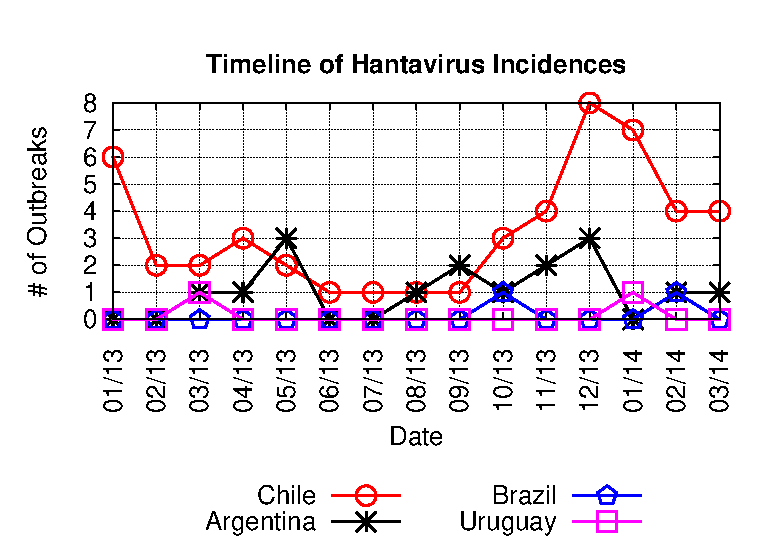
\includegraphics[trim=0 0 0 0, clip,scale=0.4]{fig/hanta_outbreaks_timeline.eps} \label{fig:hanta_timeline}}
        \subfigure{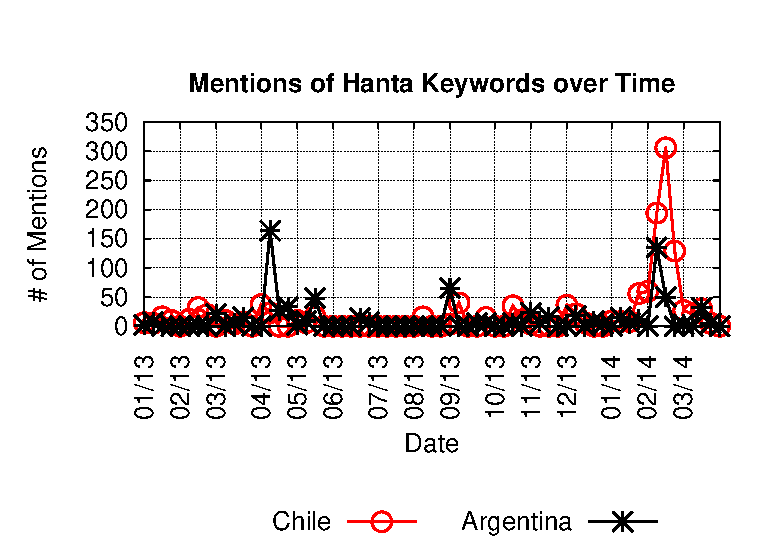
\includegraphics[trim=0 0 0 0, clip,scale=0.4]{fig/hanta_timelines_Chile.eps} \label{fig:hanta_timelines_ch}}
        \subfigure{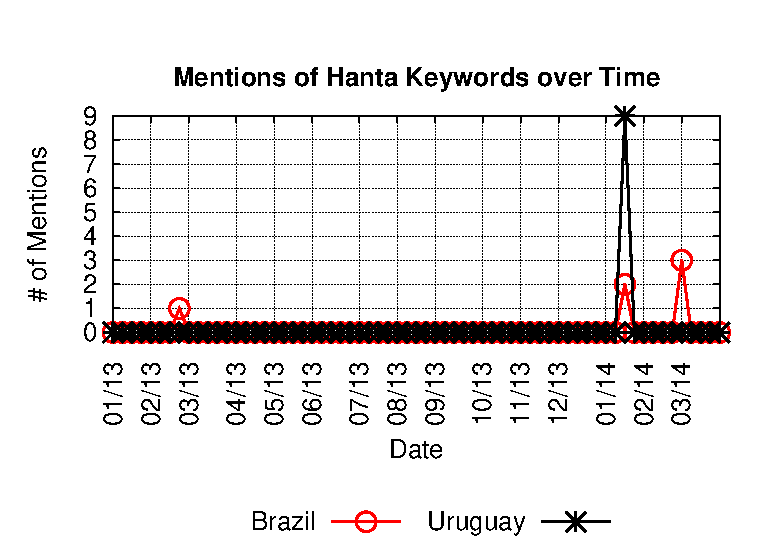
\includegraphics[trim=0 0 0 0, clip,scale=0.4]{fig/hanta_timelines_Brazil.eps} \label{fig:hanta_timelines_br}}
\end{center}
\caption{Timeline of hantavirus outbreaks from January 2013 to March 2014 for Chile, Argentina, Brazil and Uruguay. No hantavirus outbreaks were reported for other countries in Latin America.}
\label{fig:hanta_timelines}
\end{figure*}

The second challenge is that different data sources may exhibit different delays at reporting rare disease incidences, and using their data for predicting outbreaks may lead to predictions of significantly different accuracies. 

\begin{example}
We continue with the previous scenario and consider using each data source in isolation for predicting hantavirus outbreaks in Chile, Argentina, Brazil and Uruguay. \Cref{fig:src_char} shows the source accuracy histograms for Chile and Brazil. As shown, the accuracy levels of different data sources vary significantly. Similar results were observed for Argentina and Uruguay but omitted due to space limitations. The model used for predicting outbreaks is described in \Cref{sec:pred}.
\end{example}

\begin{figure*}[ht]
\begin{center}
        \subfigure{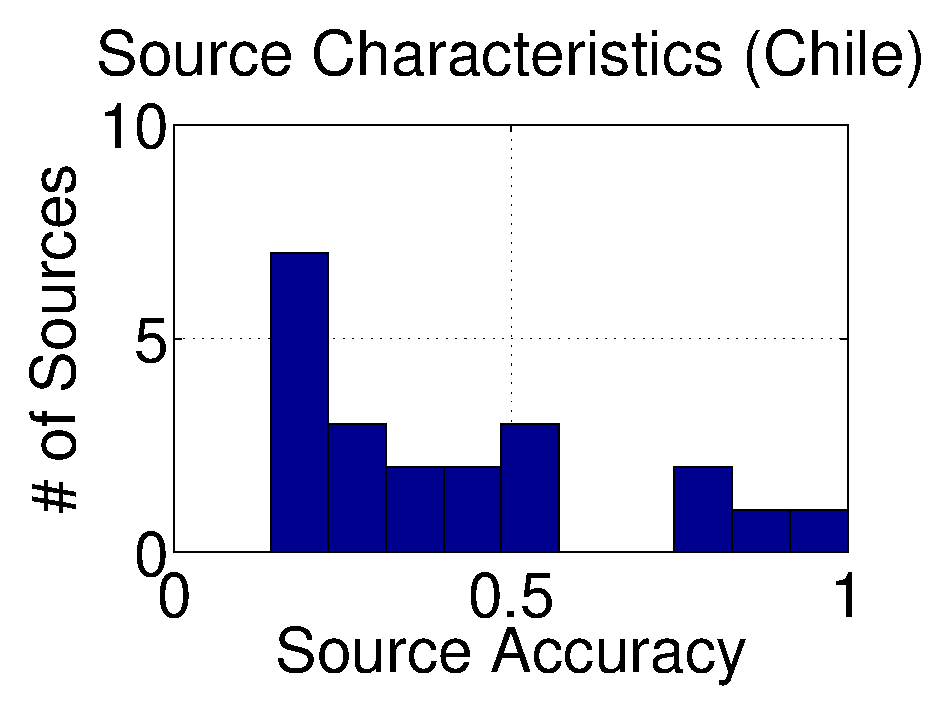
\includegraphics[clip,scale=0.2]{fig/chile_src.eps}  \label{fig:chile_src}}
        \subfigure{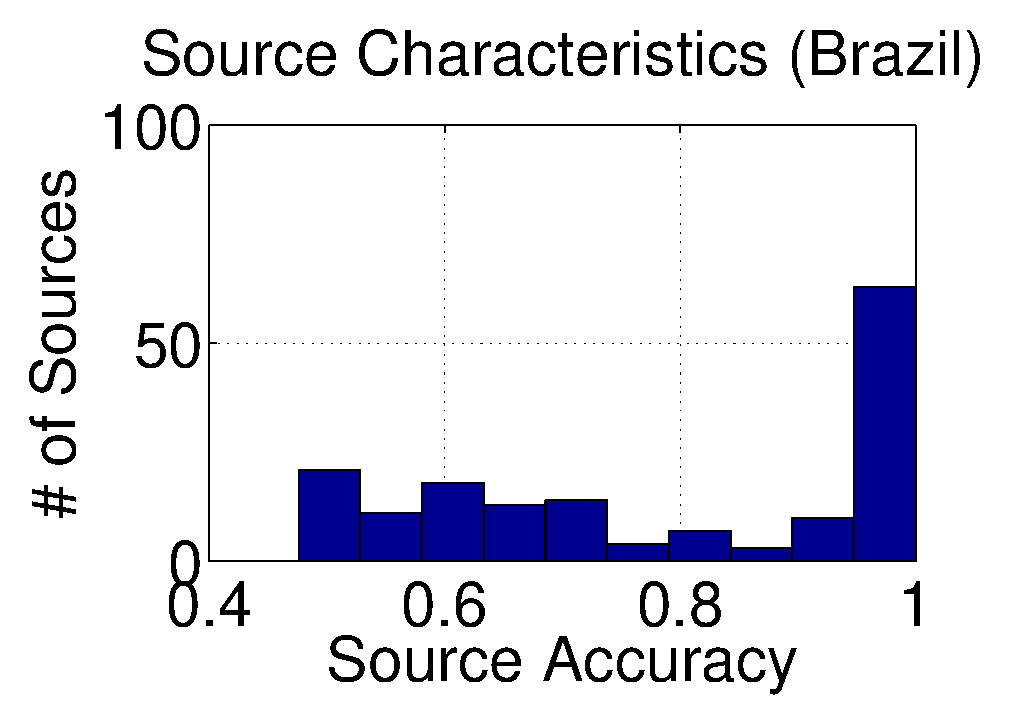
\includegraphics[clip,scale=0.2]{fig/brazil_src.eps} \label{fig:brazil_src}}
\end{center}
\vspace{-10pt}
\caption{Source accuracy histograms for Chile and Brazil.}
\vspace{-10pt}
\label{fig:src_char}
\end{figure*}


\subsection{Contributions}
\label{sec:contr}

Motivated by these examples we study the problem of forecasting disease rare outbreaks across different locations by analyzing a dynamic corpus of publicly available news articles updated at fixed intervals. We introduce \fullmodel, a novel rare disease outbreak prediction framework that consists of two major components: (a) analysis of past data to detect disease spatio-temporal patterns and (b) prediction of future outbreaks. 

Since analyzing keyword mentions over time is not sufficient to discover the temporal patterns rare disease outbreaks may exhibit, we choose to use topic models to discover the word co-occurrence patterns in the available news articles in an automated fashion. We model data sources as {\em evolving documents} over time, and introduce a new spatio-temporal topic model (\Cref{sec:model}) that explicitly models time and location jointly with word mentions. To exploit the fact that different sources exhibit different levels of accuracy when predicting rare disease outbreaks, we combine the proposed topic models with source-based anomaly detection techniques considering each source as an individual expert and fuse the individual source predictions in a single final prediction. We use anomaly detection techniques since for many locations no outbreaks may be reported in the available news articles, and hence, we require a prediction technique that can detect  unknown patterns.

The specific contributions of our approach are:
\squishlist
\item {\em Effectiveness:} \fullmodel operates on large collections of news articles and can clearly rare disease topics and their corresponding spatio-temporal patterns.
\item {\em Diversity:} Our model enables rare-disease forecasting for a diverse set of locations with significantly different outbreak patterns under a unified scheme. 
\item {\em Accuracy:} As we illustrate in an extensive experimental evaluation, considering the spatial focus and accuracy of each data source offers improved accuracy in forecasting disease outbreaks as opposed to analyzing the input of all sources for a specific location in a collective manner. 
\item{\em Forecasting instead of detecting:} \fullmodel is able to forecast outbreaks several days before they occur with a significant {\em lead-time} over reporting in news media. 
\squishend

The remainder of the paper is organized as follows: (a) we first introduce the problem of rare disease forecasting in the presence of multiple sources (\Cref{sec:problem}), (b) we then present the spatio-temporal topic model component of our framework (\Cref{sec:model}), (c) and the proposed disease prediction model  (\Cref{sec:pred}), (d) followed by an experimental evaluation (\Cref{sec:exp}) of the proposed framework on forecasting hantavirus outbreaks in Latin America. 


%\section{Introduction}
%\label{sec:old_intro}
%\todo{Lise: intro too long, a lot of details on background and approach. Moreover, redefine STAT and S-STAT more clearly}.
%There has been a growing interest in developing statistical models for detecting infectious diseases outbreaks to enable effective control measures to be taken in a sufficiently timely fashion. Most early approaches targeted specific diseases and relied on highly specialized data, including medical records or environmental time series~\cite{wong:02,wong:03}.  Recently, however, there has been a growing interest in monitoring disease outbreaks using publicly available data on the Web, including news articles~\cite{brownstein:2008,linge:09}, blogs~\cite{corley:10}, search engine logs~\cite{ginsberg:09} and micro-blogging services, such as Twitter~\cite{culotta:2010}. Due to their volume, ease of availability, and citizen participation, such {\em open source indicators} have been shown to be quite effective at monitoring disease emergence and progression.
%
%Most of the proposed techniques rely on identifying keywords related to a set of predefined diseases and detect anomalous keyword mention patterns. While effective at detecting outbreaks of common diseases, such as influenza, the above techniques have significant limitations at predicting outbreaks of {\em rare}, yet deadly, diseases, such as hantavirus. Since rare disease incidences are scarce, related keywords are sparsely distributed over time. Thus, it is difficult for keyword-based techniques to identify temporal patterns and detect the emergence of outbreaks in a timely manner. To address this limitation, researchers have employed models that identify temporal trends over {\em groups of words}, such as temporal topic models~\cite{paul:11} or frequent word-set mining~\cite{parker:13}. Both approaches rely on detecting co-occurrence patterns of word-sets over time to discover the emergence and track the evolution of diseases. 
%
%Most of the aforementioned approaches are mainly used to detect generic disease trends and focus on discovering trends within a set of closely correlated locations, i.e., regions within a specific country and not across countries. However, rare disease topics may follow significantly different patterns when considering diverse locations. For example, hantavirus outbreaks are more prominent in the Americas as opposed to Europe, and more notably, the rate of outbreaks across countries in the Americas varies significantly~\cite{jonsson:10}. Thus, not modeling the spatial correlations among disease outbreaks can confound outbreak patterns and result in unclear and sub-optimal location specific outbreak predictions. 
%
%Finally, when analyzing publicly available data from multiple sources, it is of high-importance to take into account the quality (i.e., accuracy or authoritativeness) of each source when predicting disease outbreaks. For example, when monitoring and forecasting hantavirus incidences in Chile, considering only data provided by localized sources, such as local news papers, may lead to higher accuracy than aggregating all hantavirus-related news articles by sources across the world. Nonetheless, all previous approaches assume that all sources (e.g., blogs or Twitter users) have the same accuracy and aggregate the available data when forecasting an outbreak. 
%
%In this paper, we focus on the problem of location-specific disease outbreak predictions across a diverse set of locations by analyzing a dynamic corpus of publicly available news articles. We assume a stream of news articles updated every week, and our goal is to analyze news articles up to a certain week to predict disease outbreaks for the forthcoming week. Under this scenario the problem of predicting outbreaks can be decomposed in two major components: (a) that of analyzing past data to detect spatio-temporal patterns over the available news articles and (b) that of predicting new outbreaks for the forthcoming week \todo{Lise: maybe not commit to weeks, introduce later}. To address the aforementioned problems we introduce a novel combination of source-based anomaly detection techniques with topic models.
%
%To analyze the content of past news articles, we model data sources as {\em evolving documents} over time, and introduce a {\em Spatio-TemporAl Topic} model (\model) that explicitly models time and location jointly with word co-occurrence patterns.  At a high-level the model's generative process is as follows: Each data source article is associated with an observed location. A per-location multinomial distribution over topics is sampled from a Dirichlet prior and a topic is sampled by the topic multinomial distribution corresponding to the assigned location; next two different per-topic multinomials generate the word and time point associated with each entry. \model naturally captures the fact that topics exhibit different prominence levels at different locations and different time points. 
%
%To predict a disease outbreak at a certain location, we consider each source as an independent expert.  In conjunction with \model, we learn the correlations between location and sources, and use these correlations with the output of the topic model to estimate the {\em topic focus} of each source at future time points.  We use one-class SVMs~\cite{schoelkopf:99} over the estimated topic focus of each source, to detect any per source anomalous topic prominence that constitutes an early indicator of the onset of an outbreak. Finally,  we fuse the individual source predictions into a single final prediction using weighted majority voting where a multiplicative weights algorithm~\cite{arora:2012} is used to learn the vote weight of each source. The aforementioned approach, referred to as \fullmodel, naturally captures the fact that most data sources, such as news papers, provide sufficient coverage only for a specific set of locations that is fixed over time.
%
%The main contributions of our proposed method are as follows:
%\squishlist
%\item {\em Effectiveness:} \fullmodel operates on large collections of news articles and can clearly identify topics related to rare diseases, as well as, the topic spatio-temporal patterns present in the available news articles. 
%\item {\em Diversity:} Our model enables rare-disease forecasting for a diverse set of locations with significantly different outbreak patterns under a unified scheme. 
%\item {\em Accuracy:} As we illustrate in an extensive experimental evaluation, considering the spatial focus and accuracy of each data source offers improved accuracy in forecasting disease outbreaks as opposed to analyzing the input of all sources for a specific location in a collective manner. 
%\squishend
%
%The remainder of the paper is organized as follows: (a) we first provide an overview of the problem of rare disease forecasting by analyzing data from multiple sources (\Cref{sec:problem}), (b) we then present the \model topic model ( \Cref{sec:model}), (c) and the proposed disease prediction model \fullmodel (\Cref{sec:pred}), (d) followed by an experimental evaluation (\Cref{sec:exp}) on the effectiveness of the proposed framework for forecasting hantavirus outbreaks in Latin America. 

\section{Forecasting Rare Disease Outbreaks Using Multiple Sources}
\label{sec:problem}
We assume a continuously updated collection of time-stamped event articles from a collection of data source $S$, referring to a set of locations $L$, containing words from a vocabulary $V$. We consider a discretization of time and assume that new data entries are added in batches over intervals of fixed time. For example, these time intervals may correspond to a specific day or week. For the remainder of the paper we consider a time granularity of one week, defined as the 7-day period from Sunday to Saturday referred to as an {\em epidemiological week}, or {\em epi-week} for short. 

Due to this discretization, any instance of the data collection corresponds to a fixed discretized time window up to time point $T$, and each data entry is associated with a single time point in $\{1, \dots,T\}$. It is convenient to convert this input to a collection of tuples of the form {\em (source, location, word, time point; count)} where the count corresponds to the total number a specific word was mentioned in all articles associated with the source, location and time point in the tuple. For example, a tuple (``www.biobiochile.cl'', (``Los Lagos", ``Chile"), ``hanta", ``28''; 35) means that the word ``hanta" was mentioned 35 times in all articles referring to the state of Los Lagos in Chile over the epi-week 28 provided by source ``www.biobiochile.cl''.  

Given a time point $T$, we partition the data across different sources in $S$ and view each source $s \in S$ as a {\em time-evolving document} consisting of a collection $N_s$ of time-stamped tuples, each associated with a certain {\em latent topic}. Finally, let $\mathcal{X}$ denote the set of all tuple collections $N_s$ for all sources $s \in S$ until time point $T$. Assuming a set of tuple collections $\mathcal{X}$ that get updated with time, our goal is to predict potential disease outbreaks for all locations present in the input data for the future time point $T+1$. Finally, we assume access to a gold-standard report (GSR) providing ground truth information for disease outbreaks at locations in $L$ for time points $t \prec T$. We consider GSR being updated at a much lower rate than that of $\mathcal{X}$ and therefore we can observe significant delays at obtaining ground truth information. Given the assumptions presented above, we decompose this problem into two problems:
\squishlist
\item {\bf Topic and Pattern Discovery.} Find the hidden topics that best summarize the input $\mathcal{X}$, their temporal patterns and prominence for each specific location.
\item {\bf Predicting Disease Outbreaks.} Estimate the future topic focus for each source-location pair, and use each source as an individual expert to forecast disease outbreaks. Sources may exhibit different accuracies that can be learnt comparing their predictions with the GSR.
\squishend
In the next sections, we analyze the two main components of \fullmodel addressing the aforementioned problems.

\section{Spatio-temporal Topic Models}
\label{sec:model}
The first component of \fullmodel deals with the topic and pattern discovery problem.  We introduce a topic model that explicitly models time and location jointly with the word co-occurence patterns over news articles from multiple data sources. We start by reviewing the basic Latent Dirichlet Allocation (LDA) model~\cite{blei:2003}. 

LDA is a Bayesian network that generates a document using a mixture of topics. In its generative process, for each document $d$, a multinomial distribution $\theta_d$ over topics is randomly sampled from a Dirichlet with parameter $\alpha$, and then to generate each word, a topic $z_{di}$ is chosen from this topic distribution, and a word, $w_{di}$, is generated by randomly sampling from a topic-specific multinomial distribution $\phi_{z_{di}}$. 

\vspace{-15pt}\begin{table}[h]
\small \centering
\caption{Notation used in this paper.}
\begin{tabular}{c l}
\hline
{\bf Symbol} & {\bf Description}  \\
\hline
K & Number of topics  \\
S & Number of sources \\
V & Number of words \\
T & Number of discrete time-points \\
L & Number of locations \\
$N_s$ & Number of entries in each source $s$\\
$\theta_l$ & Topic multinomial distr. for location $l$\\
$\phi_z$ & Word multinomial distr. for topic $z$\\
$\xi_z$ & Time point multinomial distr. for topic $z$\\
$z_{si}$ & Topic of the $i$th entry from source $s$ \\
$l_{si}$ & Location of the $i$th entry from source $s$ \\
$w_{si}$ & Word of the $i$th entry from source $s$ \\
$t_{si}$ & Time point of the $i$th entry from source $s$ \\
\hline
\end{tabular}
\label{tab:notation}
\end{table}
\vspace{-5pt}

Our proposed spatio-temporal topic model uses location and topic specific distributions to model the generation of words and timestamps. Topic discovery is influenced not only by word co-occurences, but also spatial and temporal information. Our notation is summarized in \Cref{tab:notation}, and the graphical model representation of the model is shown in \Cref{fig:stm_model}.  Next, we describe the model's generative process for the word and time point of each entry corresponding to an observed location.

\begin{figure}[h]
\begin{center}
       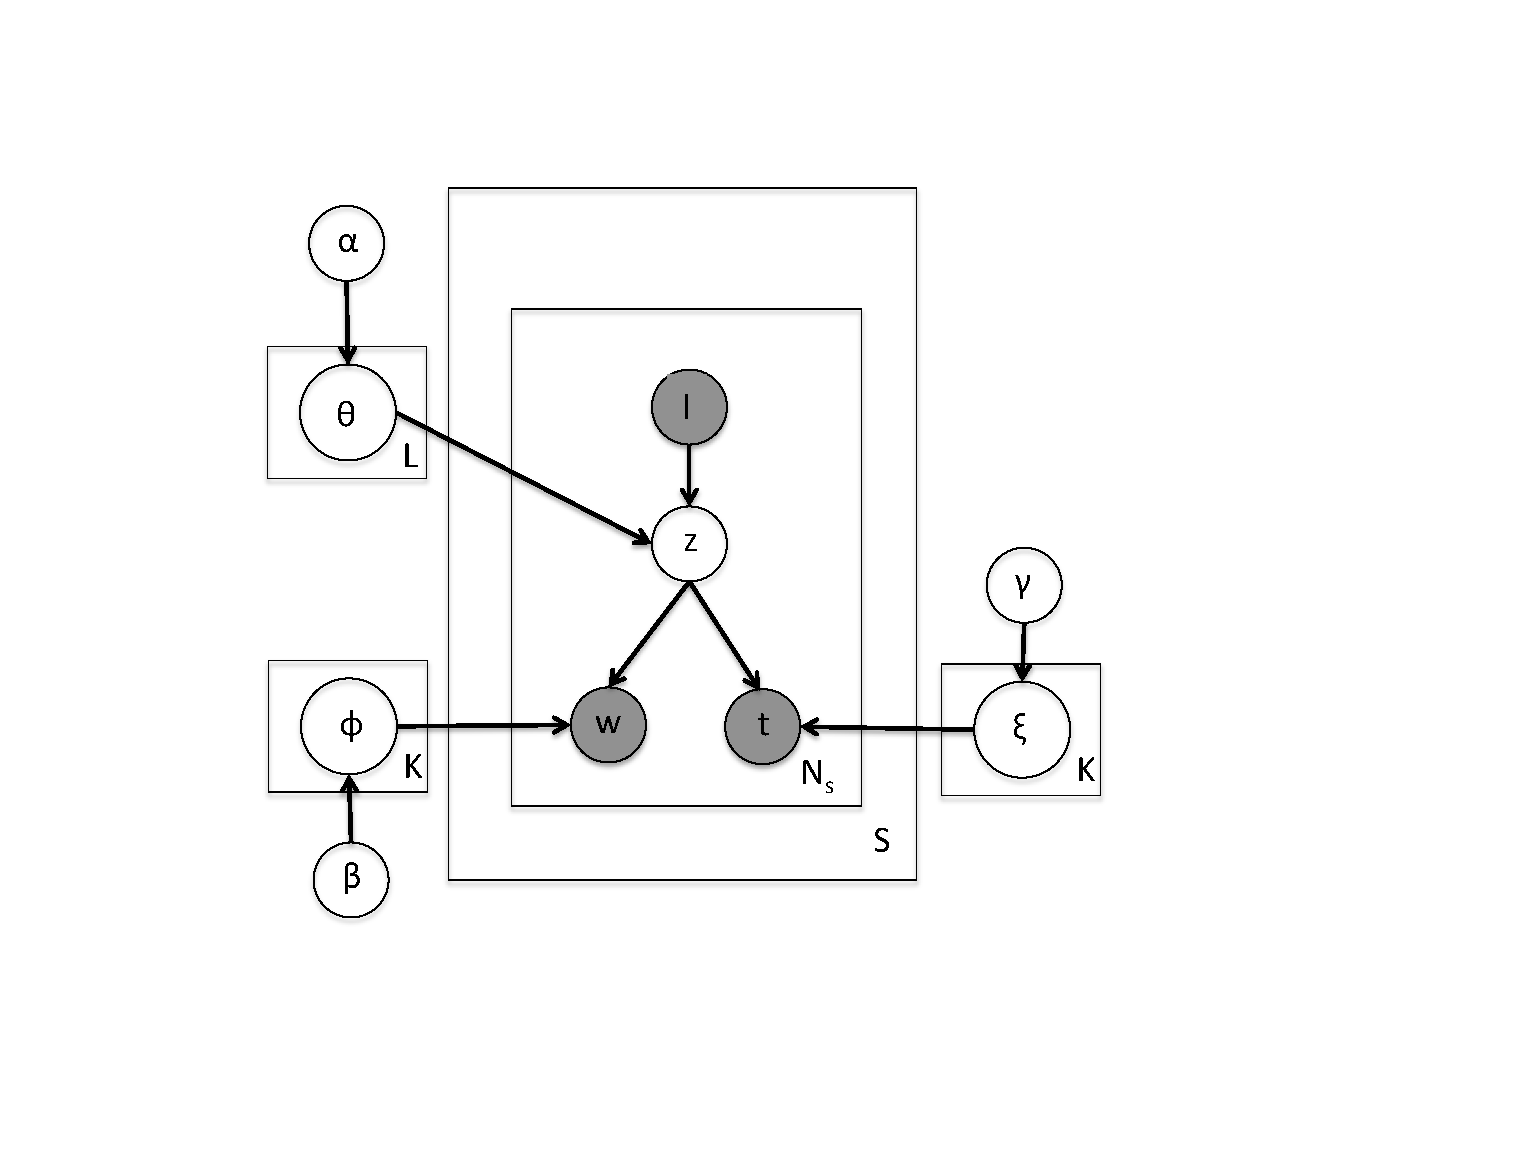
\includegraphics[trim = 30mm 35mm 70mm 25mm, clip, scale=0.3]{fig/stm_model.eps} \label{fig:stm_model}
\end{center}
\caption{Plate notation for the proposed spatio-temporal topic model.}
\vspace{-10pt}
\label{fig:stm_model}

\end{figure}
\vspace{-10pt}\ \\{\bf \model generative proceess}
\begin{enumerate}[noitemsep]
\item Draw $K$ multinomials $\phi_z\sim\mbox{Dir}(\beta)$ for each topic $z$
\item Draw $K$ multinomials $\xi_z\sim\mbox{Dir}(\gamma)$ for each topic $z$
\item Draw $L$ multinomials $\theta_l\sim\mbox{Dir}(\alpha)$ for each location $l$
\item For each source  $s \in S$ and entry $i \in N_s$ with $l_{si}$:
\begin{enumerate}[noitemsep,nolistsep]
\item Draw a topic $z_{si}$ from the multinomial $\theta_{l_{si}}$
\item Draw a word $w_{si}$ from multinomial $\phi_{z_{si}}$
\item Draw a time-point $t_{si}$ from multinomial $\xi_{z_{si}}$
\end{enumerate}
\end{enumerate}

Each source entry is associated with a location $l_{si} \in L$ and we consider a distribution $\theta_{l_{si}}$ over topics that is randomly sampled from a Dirichlet with parameter $\alpha$. To generate each entry $i \in N_s$ for source $s$, first, a topic $z_{si}$ is chosen from the topic distribution $\theta_{l_{si}}$, and then, a word $w_{si}$ and time-point $t_{si}$ are generated by randomly sampling from the topic-specific multinomial distributions $\phi_{z_{si}}$ and $\xi_{z_{si}}$.  In our experiment we assume a fixed number of topics $K$.

We use Gibbs sampling to perform approximate inference. Using a Dirichlet conjugate prior for the multinomial distributions allows us to easily integrate out $\theta$, $\phi$ and $\xi$.  To estimate the model parameters, we calculate the conditional probability distribution $\Pr(z_{si}|{\bf w},{\bf t}, {\bf l}, {\bf z}_{-si}, \alpha, \beta, \gamma)$ where ${\bf z}_{-si}$ represents the topic assignments for all entries in $s$ except the $i$-th entry. We have: \vspace{-10pt}

{\small \begin{align}
\label{eq:conditional}
&\Pr(z_{si}| \w,\tim,\loc,\z_{-si};\alpha,\beta,\gamma) \propto \frac{n^{k,-(s,i)}_{w_{si}} + \beta_{w_{si}}}{\sum_{r = 1}^V n^{k,-(s,i)}_{r} + \beta_{r}}  \nonumber \\
& \cdot \frac{m^{k,-(s,i)}_{t_{si}} + \gamma_{t_{si}}}{\sum_{t = 1}^T m^{k,-(s,i)}_{t} + \gamma_{t}} \cdot \frac{o^{k,-(s,i)}_{l_{si}} + \alpha_{l_{si}}}{\sum_{l = 1}^L o^{k,-(s,i)}_{l} + \alpha_{l}}
\end{align}}

\noindent where $n^{z}_{r}$ denotes the number of times word $r$ was associated with topic $z$ across all sources and entries, $m^{z}_{t}$ denotes the number of times time-point $t$ was associated with topic $z$ across all sources, $o^z_l$ denotes the number of times location $l$ was associated with topic $z$ across all sources and their entries, and $-si$ in the superscript indicates that the current example has been excluded by the count summations. The derivation of the Gibbs sampling algorithm is shown in \Cref{sec:gibbs}. Once the sampler has converged, we estimate the parameters of the multinomials $\theta$, $\phi$, and $\xi$ as follows:
{\small \begin{align}
\label{eq:updates}
\theta_{l,z} = \frac{o^z_l + \alpha_l}{\sum_{z=1}^K o^z_l + \alpha_l} \nonumber \\
\phi_{z,v} = \frac{n^z_l + \alpha_l}{\sum_{v=1}^V n^z_v + \beta_v}  \\
\xi_{l,z} = \frac{m^z_t + \alpha_l}{\sum_{t=1}^T m^z_t + \gamma_t} \nonumber
\end{align}}
For each entry in a set of event collection $\mathcal{X}$ we assign a hidden topic $z$ according to \Cref{eq:conditional}, and update the appropriate counts. After the sampling, we compute the distributions ${\boldsymbol \theta}$, ${\boldsymbol \xi}$ and ${\boldsymbol \phi}$ according to equation \Cref{eq:updates}.   

\section{Source-based Disease Outbreak Prediction}
\label{sec:pred}
The second component of \fullmodel is responsible for forecasting outbreaks at a future time point $t$ for each of the locations present in $\mathcal{X}$. At a high-level, for each location $l$, we extract an individualized prediction from each source that is relevant to $l$ and fuse the individual predictions using weighted majority voting. We learn the corresponding weights using a multiplicative weights update algorithm.

\subsection{Predicting Disease Outbreaks with a Single Source}
\label{sec:source_pred}
Detecting an anomaly in the content of source $s$ for location $l$, requires reasoning about the relevance of the source's content to the discovered disease topics. We view this problem as an instantiation of the {\em document classification}~\cite{strehl:2000} problem and show how the relevance between the content of a source and a topic can be measured using {\em cosine similarity}.

For each topic $z \in K$, we have a distribution $\phi_z$ over all words in the vocabulary $V$. Following a similar approach to Matsubara et al.~\cite{matsubara:2012}, we extract the average occurrence rate $\bar{x}_w$ for each word $w \in V$ across all entries and construct an {\em average representative document} for each topic $z \in Z$, characterized by a vector $F_z$ that contains the expected occurrence frequency of each word $w \in V$ given the topic. We define the $w$-th entry of $F_z$ corresponding to word $w$ as $F_z,w = \bar{x}_w \cdot \phi_{z,w}$. Similarly, given a source $s$,  a location $l$ and a time point $t$, the content of a source is described with a word frequency vector $F_{s,l,t}$. Given the vectors $F_z$ and $F_{s,l,t}$ we define the relevance of the content of source $s$ for location $l$ at time $t$ to topic $z$ as:
{\small \begin{equation}
{\sf Relevance}(s,z;l,t) = {\sf CosineSimilarity}(F_{s,l,t},F_z)
\end{equation}}
where the cosine similarity of two vectors $A$ and $B$ is:
{\small \begin{equation}
{\sf CosineSimilarity}(A,B) = (A \cdot B)/(\|A\| \|B\|)
\end{equation}}\vspace{-10pt}

However, we want to predict disease outbreaks at future time points when the content of each source is not available to us. Therefore, given a source $s$, a location $l$ and a future time point $t$, we estimate the entries of $F_{s,l,t}$ considering the expected frequency of each word. Let $\hat{F}_{s,l,t}[w]$ denote the expected frequency for word 
$w \in V$. To compute the expected frequency $\hat{F}_{s,l,t}[w]$, we need to consider the conditional probability of source $s$ mentioning word $w$ at a future time point $t$, denoted by $\Pr(t|s,w)$, the conditional probability of source $s$ publishing word $w$ in an article related to the location $l$, denoted by $\Pr(w|s,l)$, and 
the probability of word $w$ being generated by any topic $z \in K$, given location $l$ and time point $t$. 
We have that:
{\small \begin{equation}
  \hat{F}_{s,l,t}[w] = \bar{x}_{w} \cdot \Pr(t|s,w) \cdot \Pr(w|s,l)\cdot \sum_{z \in K}\phi_{z,w}\cdot \theta_{l,z} \cdot \xi_{z,t}
\end{equation}}

\noindent where $\bar{x}_{w}$ denotes the average rate of occurrences of word $w$ in $\mathcal{X}$,  and 
$\phi_{z,w}$, $\theta_{l,z}$, and $\xi_{z,t}$, can be retrieved by the output of the topic model component of \fullmodel.  Given the historical data, we estimate the probability $\Pr(w|s,l)$ with its maximum likelihood as:
{\small \begin{equation}
  \Pr(w|s,l) = \frac{n_{w,s,l}}{\sum_{w\in V}n_{w,s,l}}
\end{equation}}

\noindent where $n_{w,s,l}$ denotes the number of mentions of word $w$ from source $s$ in location $l$.
Notice that $\xi_{z,t}$, i.e., the probability of topic $z$ being prominent at time $t$, 
and $\Pr(t|s,w)$ correspond to future time points and need to be estimated.  

According to the problem description in \Cref{sec:problem}, the available historical 
data spans up to time point $t-1$. Thus, we estimate the probability of the source 
mentioning a particular word $w$ at a future time $t$ by considering the weighted average occurrence rate of word $w$ in the source:
{\small \begin{equation}
\Pr(t|s,w) = \frac{\sum_{\tau = 1}^{t-1} \frac{1}{t - \tau}I(\tau,s,w)}{\sum_{\tau = 1}^{t-1} \frac{1}{t - \tau}}
\label{eq:prob_time}
\end{equation}}

\noindent where $I(s,\tau,w)$ is an indicator variable equal to one if source $s$ mentioned word $w$ at least once at time $\tau$, and zero otherwise. 
To estimate the probability $\xi_{z,t} \mbox{ with } z \in \{1, 2, \dots, K\}$, 
we use the values of distribution $\xi_{z}, \forall z \in K$ corresponding to past time points. In particular, we use an autoregressive model over the values of topic $z$ for the $n$ previous time intervals, denoted by $\xi_{z,t-1},\xi_{z,t-2},\dots,\xi_{z,t-N}$:
{\small \begin{equation}
\xi_{z,t}=a_1 \cdot \xi_{z,t-1}+a_2\cdot \xi_{z,t-2}+\dots +a_n\cdot \xi_{z,t-n}
\vspace{-10pt}
\end{equation}}

\noindent where $a_1,a_2,.....,a_n$ are the regression coefficients.  We compute the source-topic relevance for each source-location and topic combination using the aforementioned techniques.

Since rare disease incidences are scarce over time. Therefore, the source-topic relevance values for a rare disease topic will be low for most time points and high only for few time points corresponding to an outbreak. Following this observation, high relevance values for a rare disease topic, can be viewed as anomalous points, and thus, anomaly detection techniques can be used to identify if the source-topic relevance corresponds to an anomalous point.

We use one-class SVMs~\cite{schoelkopf:99} (OCSVM) to classify the source-topic relevance values as anomalous or not. OCSVMs have successfully been used in a variety of anomaly detection tasks~\cite{manevitz:2002,steinwart:05, heller:03}. Furthermore, OCSVMs present superior performance compared to other anomaly detection techniques, such as Nearest Neighbor classification, in scenarios where a small number of anomalous example is available~\cite{khan:13}. Finally, OCSVMs do not make any assumptions on the distribution of the data points.

%A OCSVM maps input data $X$ into a high dimensional feature space $H$ via a kernel $\Phi: X \rightarrow H$ and finds the maximal margin hyperplane which best separates the training data from the origin. The classification rule corresponds to $f(x) = {\sf sign}(\mathbf{w}\Phi(x) - b)$, where $\mathbf{w}$ is a weight vector and $b$ is a bias term. We use this classification rule to detect if a new point $x$ is an anomalous point (i.e., $f(x) < 0$). 

To predict outbreaks for a future time point $t$, we train a separate OCSVM for each source-location pair $(s, l)$ using the source-topic relevance values for all time points up to $t-1$ as training data.  The training entry for a time point $t^{\prime} \prec t$ corresponds to a vector $<{\sf Relevance}(s,z_1;l,t^{\prime}), {\sf Relevance}(s,z_2;l,t^{\prime}), \dots>$ containing the relevance values for all topics $z_1, z_2, \dots$ that are relevant to the rare disease under consideration. 

\subsection{Fusing Multiple Predictions}
\label{sec:integration}
Our final goal is to forecast the incidence of a particular disease for a specific location, thus, we fuse the predictions of all sources into a single prediction for each location $l \in L$ at time $t$. We use a weighted majority voting algorithm based on the multiplicative weights update framework\cite{arora:2012}.

Given time $t$ in the future, we focus on a location $l$ and view each source $s \in S$ as an expert providing a prediction $d_s \in [-1,1]$ with the value $-1$ corresponding to the emergence of an outbreak and $1$ otherwise. We assign a weight $w_s$ to each source, and given the predictions of all sources, we predict yes/no for an outbreak at location $l$ by taking the majority vote $\sum_{s \in S} w_s \cdot d_s$.  We learn weights $w_s$ using the multiplicative weights algorithm shown in Alg. \ref{algo:mw}.

\begin{algorithm}[h]
\caption{Multiplicative Weights Update for Sources}
{\footnotesize \begin{algorithmic}[1]
\STATE {\bf Input:} $S_l$: set of sources for location $l$; ${\bf D_l}$: training points; $R_{S_l}$: source-topic relevance dictionary for sources in $S_l$ and points in ${\bf D_l}$; $O_{S_l}$: one-class SVMs for $S_l$; $\epsilon$: discount factor
\STATE {\bf Output:} $\bf{W}$: weights for sources in $S_l$
%\STATE $T \leftarrow \lceil \frac{4\ln(|N_l|)}{\epsilon^2} \rceil$ {\em /* Initialize number of epochs */}
\STATE Initialize all weights $W$ to 1
\FORALL {$d \in {\bf D_l}$}    	
	\FORALL {$s \in S_l$}
	\STATE {\em /*Extract the expert's vote*/}
	\STATE $v \leftarrow O_{S_l}[s].predict(R_{S_l}[s][d])$
	\IF {v is wrong}
		\STATE  $W_k \leftarrow W_k\cdot \exp(-\epsilon)$ {\em /* Decrease the weight */}
	\ELSE
		\STATE $W_k \leftarrow W_k\cdot \exp(\epsilon)$ {\em /* Increase the weight */}
	\ENDIF
	\ENDFOR	
	\STATE Normalize the weights to sum up to $1.0$
\ENDFOR
\RETURN ${\bf W}$
\end{algorithmic}}
\label{algo:mw}
\end{algorithm}

Consider a location $l$. To construct the necessary input for the multiplicative weights update algorithm, we: (i) identify the set of sources $S_l$ relevant to location $l$, i.e., sources that have published for location $l$, and (ii) construct the set of training points  ${\bf D_l}$ by considering the reported outbreaks in GSR (\Cref{sec:problem}) for location $l$ and the disease under consideration. We populate ${\bf D_l}$ with tuples of the form $(time point, outbreak)$ for all historical time points up to the latest time point present both in $\mathcal{X}$ and GSR and set the value of $outbreak$ to $-1$ if an actual outbreak was reported and $1$ otherwise. Finally, we use the past source-topic relevance values for the sources in $S_l$ and the training points in ${\bf D_l}$.

Given the input described above, the algorithm proceeds in an iterative fashion updating the weights of the sources considering the accuracy of their predictions. More precisely, the algorithm iterates over all training points in ${\bf D_l}$ (Ln. 4).  At each iteration, it examines all available sources (Ln. 5) and extracts their prediction corresponding to a specific training point from the past (Ln. 6-7). If the expert is mistaken, it's corresponding weight is reduced in a multiplicative fashion (Ln. 9), otherwise its weight is increased (Ln. 11). Finally, the algorithm outputs the normalized weights, which are later used to fuse the individual source predictions for future time points. The process is repeated as more ground-truth data are becoming available in GSR.

Finally, we associate each outbreak prediction for location $l$ with a {\em confidence score}. Let $S$ be the set of relevant sources for location $l$ and $S_{-1}$ be the subset of sources predicting an outbreak. Moreover, let $a_l(s)$ be the overall {\em accuracy} of a source $s \in S_l$ considering its past predictions for location $l$. The accuracy of source $s$ is defined over the available past time window as $a_l(s) = \frac{\#\mbox{ correct predictions}}{\#\mbox{total prediction}}$ and corresponds to the probability of $s$ giving a correct prediction. Combining the above, the confidence score is: 
{\small \begin{equation}
ConfScore = \prod_{s \in S_{-1}}a_l(s) \cdot \prod_{s \in S_l \setminus S_{-1}} (1 - a_l(s))
\label{eq:conf}
\end{equation}}

\noindent Given the confidence score of each outbreak prediction, one can use a threshold mechanism to select the final outbreak predictions, and balance the trade-off between precision and recall as we discuss in \Cref{sec:exp}. In particular, one can select to report an outbreak prediction only if it is in the $95\%$ confidence interval. Fusing the predictions of individual sources, we predict  {\em if} a disease outbreak will happen during a specific epi week. To predict the exact day of the incidence, we adopt a standard relative date within the epi-week to be the date at which the rare disease incidence will occur, and tune it using cross-validation. 


\section{Experimental Evaluation}
\label{sec:exp}
We present an empirical evaluation of the proposed framework. First, we evaluate how effective is the topic model component of \fullmodel in discovering disease topics and their spatio-temporal patterns. Then we evaluate the accuracy and quality of the prediction from the second component of our proposed framework. We empirically study these questions with real-world data focusing on rare-disease outbreaks in countries in Latin America.

% then The main questions we seek to address are: (1) how effective is the proposed topic model in identifying disease topics, and in discovering the corresponding spatio-temporal patterns, (2) how accurately can the proposed techniques forecast disease outbreaks and what is their forecast lead-time compared to traditional detection based on news mentions, and (3) whether leveraging the varying authoritativeness levels of data sources for different locations can improve the accuracy of outbreak predictions. 

\subsection{Experimental Setup}
\noindent{\bf Data:} We use a dataset corresponding to a corpus of public health-related news articles and tweets extracted from HealthMap~\cite{healthmap}, a prominent online aggregator of news articles and tweets for disease outbreak monitoring and real-time surveillance of emerging public health threats. Since, we focus on countries in Latin America the vocabulary we consider consists of Spanish and Portuguese words and does not contain only disease related words. Traditional IR pre-processing such as stop-word removal and term frequency modeling is performed over a fixed vocabulary of words. The dictionary contains words that are either commonly associated with diseases (e.g.,``contagious") or words associated with a specific disease (e.g.,``rodents",``hanta" for hantavirus). Finally, each article is associated with a data source and a location corresponding to a country-state pair.

When predicting for an epi-week $t$ we use historical (weekly) data from June 2012 up to the previous week $t-1$ to discover the topics using the model presented in \Cref{sec:model} and estimate the source-topic relevance values for $t$ at each available location. As we progress to prediction for forthcoming weeks, we gather the estimated source-topic relevance values corresponding to past weeks and align them with the gold standard report (\Cref{sec:source_pred}) to  form the necessary training points for the OCSVMs. We evaluate the performance of our proposed techniques from January 2013 to March 2014. The size of the input data varies over time, as new articles are added every epi-week. The number of words ranges from 20,908 to 48,700, the number of locations from 74 to 144 and the number of data sources from 381 to 798.

\noindent{\bf GSR:} We make use of a gold standard report (GSR) which gives ground truth determinations of whether a disease incidence (hantavirus) happened in a given location. The GSR is determined by analysts considering multiple news sources and studying bulletins issued by health reporting organizations such as ProMED~\cite{probmed}.

\noindent{\bf Models:} We evaluate the following models:
\squishlist
\item \fullmodel: Our source-based framework introduced in Sections \ref{sec:model} and \ref{sec:pred} coupled with a thresholding mechanism where for a week and country accepts only the predictions with confidence scores (\Cref{eq:conf}) in the top-$k$ percentile of all prediction scores for that country.
\item \locationmodel: A variation of \fullmodel that uses the topic model component to identify disease related topics but integrates this with a {\em location-only} anomaly detection approach. We follow an approach similar to the one introduced in \Cref{sec:source_pred}. For each location we calculate the location-topic relevance values for future time points and use an OCSVM  to detect anomalous points. To calculate the location-topic relevance, we estimate each entry of the location's word frequency vector as $\hat{F}_{l,t}[w] = \bar{x}_{w} \Pr(t|l,w) \sum_{z \in K}\phi_{z,w}\cdot \theta_{l,z} \cdot \xi_{z,t}$, where $\Pr(t|l,w)$ is defined similarly to \Cref{eq:prob_time}. Intuitively,  \locationmodel integrates news articles from multiple data sources ignoring the accuracy of individual sources. We use a thresholding mechanism similar to that of \fullmodel considering the accuracy of each state-based OCSVM. 
\item \keymodel: A {\em keyword} based prediction technique that monitors the mentions of the Hantavirus related keyword set $\{$``hanta", ``hantavirus", ``roedores", ``ratones", ``cardiopulmonar"$\}$ and uses an OCSVM to predict future outbreaks based on past mentions of words. This word-set reflects the fact that Hantaviruses have almost entirely been linked to human contact with rodent excrement and their symptoms affect the heart and the lungs.
\item BRM: A {\em base rate model} that assumes a fixed rate for the occurrence of rare disease outbreaks for each location and for each
month. To determine this rate, the model extracts the average frequency of outbreak occurrences reported over a past time window of four months. BRM reports disease outbreaks for that location at a frequency equal to the extracted rate. Alerting dates are assigned to the beginning of each month while event dates are assigned uniformly at random to a day within the corresponding month. We take the average performance over 25 independent runs.
\squishend
All models are implemented in Python and the evaluation is performed on an Intel(R) Xeon(R) CPU E7- 4870 @2.40GHz/64bit/1TB machine. 


\noindent{\bf Parameter Setup:} The OCSVM parameters are tuned using leave-one-out cross-validation. For the topic model, we set the parameters of the Dirichlet priors to $\alpha = 2/K$, $\beta = 0.01$ and $\gamma = 0.01$ where $K$ is the number of topics. We evaluated the topic model with $K = \{8, 12, 15\}$ and found that $K=12$ results in more meaningful topics.  


\noindent{\bf Metrics:} We adopt five key measures of performance. Given our predictions, we compute the precision, recall and F1-score at a country level, grouping together prediction for locations in the same country. We also compute an average warning quality for each country. Each prediction for a location in the country under consideration is assigned a quality score $Q = \frac{4}{3}(1 + a_{loc} + a_{date})$, where $a_{loc}$ and $a_{date}$ denote the location and date accuracy of the prediction. To calculate $a_{loc}$ we use a two-level topology, considering the country, and state corresponding to the location of a warning. A partial score of $0.5$ is assigned to a warning if it matches the country of an outbreak correctly and an additional score of $0.5$ is assigned if the warning matches the state correctly. The date specific accuracy $a_{date}$ is calculated as: 
\begin{equation} 
a_{date} = 1 - \frac{min(|\mbox{predicted date} - \mbox{actual date}|,7)}{7}
\end{equation} 
Finally, we consider the lead time of our predictions, which is calculated as the time between the date of alerting and the actual date of reporting the outbreak (not the incidence date of the outbreak). Notice that lead time is different from the date accuracy described above.  

\noindent{\bf Mapping Warnings to Events:} Since there could be multiple events (and/or alerts) in a given month, a strategy is necessary to map events to alerts. We conduct a maximum bipartite matching between events and alerts where (i) an edge exists if the alert was issued prior to the reporting date of the event, (ii) the weight on the edge denotes the quality score. 

\subsection{Disease Topics Discovery} \textbf{{\em How effective is the proposed topic model in identifying disease topics and their temporal patterns?}} The HealthMap corpus contains mentions to both common and rare diseases over multiple countries in Latin America. The most prevalent diseases mentioned in the dataset are avian flu (i.e., type h5n1), dengue fever, swine flu (i.e., h1n1 flu), the hantavirus pulmonary syndrome (HPS) and the hantavirus hemorrhagic fever with renal syndrome (HFRS)~\cite{jonsson:10}. 


\begin{table*}[t]
\small\centering
\caption{Three discovered topics that are related to hantavirus. The first two topics are related to the two different hantavirus syndromes (i.e., HPS and HFRS) and the third topic is related to generic information about the  transmission of the virus. Histograms show the topic prominence over time; The top words with their probability in each topic are shown.}
\begin{tabular}{|lr|lr|lr|}
\hline
\multicolumn{2}{|c|}{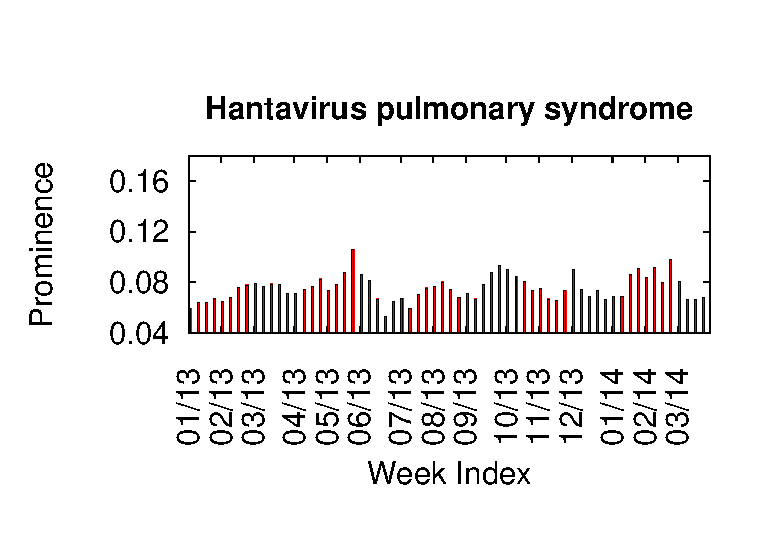
\includegraphics[clip,scale=0.4]{fig/topic_hanta_timeline.eps}} & \multicolumn{2}{|c|}{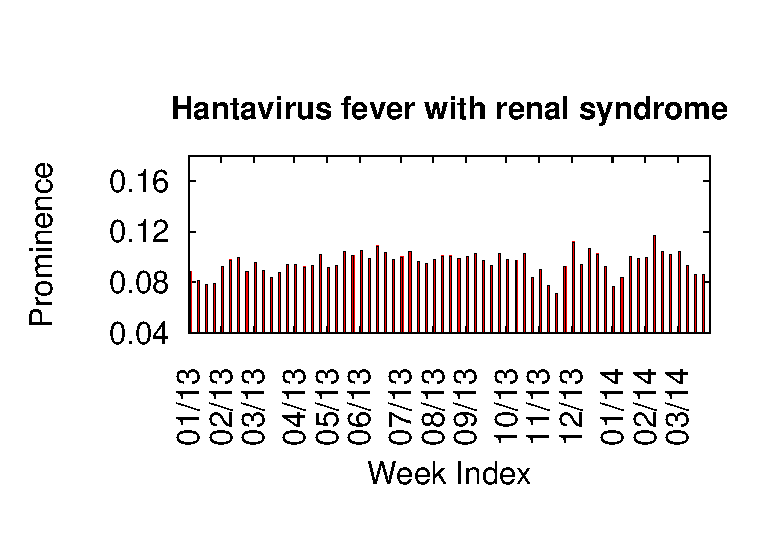
\includegraphics[clip,scale=0.4]{fig/topic_hanta3_timeline.eps}}& 
\multicolumn{2}{|c|}{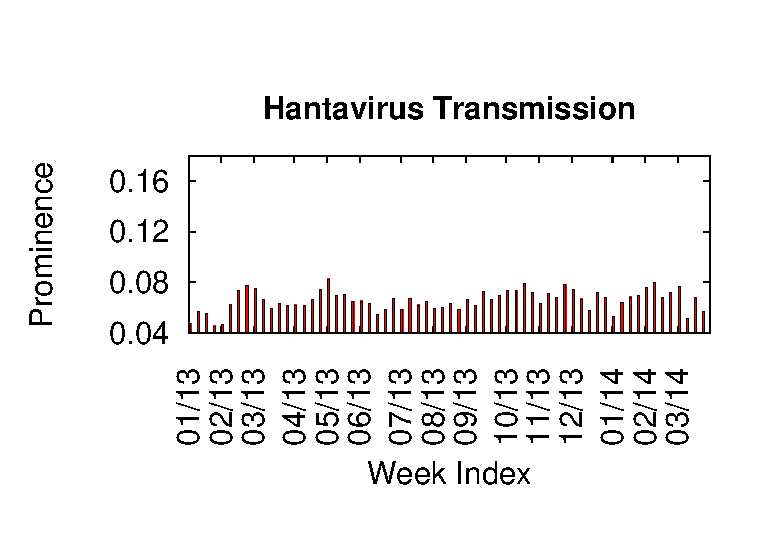
\includegraphics[clip,scale=0.4]{fig/topic_hanta2_timeline.eps}} \\ \hline
virus & 0.0468 & vacuna & 0.0057 & paciente & 0.0220 \\
epidemia & 0.0443 & campos & 0.0031 & transmissor & 0.0133 \\
enfermos & 0.0066& provincial & 0.0028  & lixo &0.0099 \\
hanta & 0.0068 & hantavirus & 0.0024  & criaderos & 0.0088\\
viral & 0.0038 & tosse & 0.0022 & respiratorias & 0.0061 \\
territorio & 0.0027 & nariz & 0.0019 & manos & 0.0056 \\
pneumonia & 0.0014 & estornudar & 0.0011 & boca & 0.0047 \\
sangre & 0.0014 & abdominal & 0.0008 & rural & 0.0038 \\
ratones & 0.0006 & lluvia & 0.0008 & musculares & 0.0028 \\
cardiopulmonar & 0.0002 & renal & 0.0005 & roedores & 0.0022 \\
\hline
\end{tabular}
\label{tab:hanta_topics}
\vspace{-10pt}
\end{table*}

While the first three diseases are widespread with a large number of incidences, hantavirus syndromes are rather rare, with a small number of incidences (\Cref{fig:hanta_timeline}) with the majority of outbreaks occurring in Chile. No seasonal patterns governing the outbreak incidences were observed for any of the countries under consideration.

%\begin{figure}[h]
%\begin{center}
%	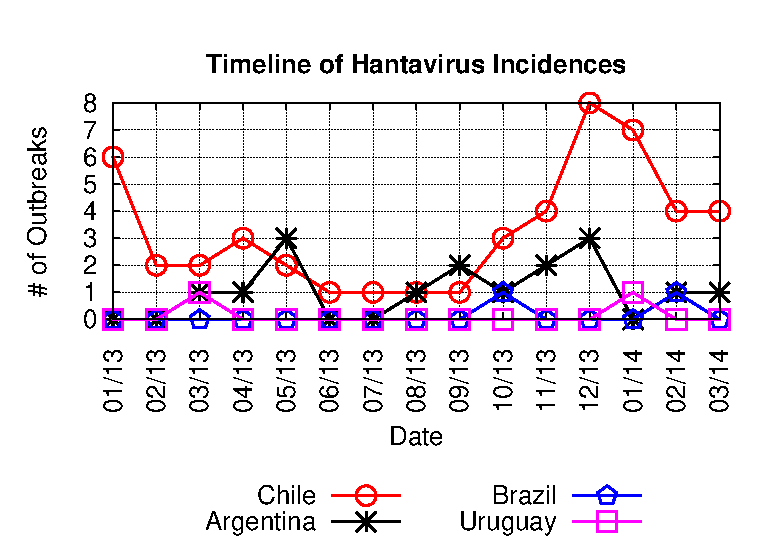
\includegraphics[trim=0 0 0 0, clip,scale=0.5]{fig/hanta_outbreaks_timeline.eps}
%\end{center}
%\caption{Timeline of hantavirus outbreaks from January 2013 to March 2014 for Chile, Argentina, Brazil and Uruguay. No hantavirus outbreaks were reported for other countries in Latin America.}
% \label{fig:hanta_timeline}
%\end{figure}

We evaluate the topics discovered by our topic model. Six out of the twelve topics are related to the diseases mentioned above, while the rest are background topics related to non-disease aspects of the news articles. We focus only on the disease related topics. To evaluate the disease topics, we consider a vocabulary of 184 health-related words. For each topic, we examine the most likely words based on the health-related vocabulary and their prominence over time. Given a time point, we define the prominence of a topic as the fraction of articles of that topic over the total number of articles published at that time point.

\Cref{tab:hanta_topics} shows three topics related to hantavirus, their most likely words based on the health-related vocabulary and their prominence histograms over time. 
The first topic refers to the HPS syndrome with words such as ``pneumonia", ``sangre" (blood), and ``cardiopulmonar" being ranked higher. We see that the proposed topic model is able to retrieve the correlation between words ``hanta" and ``ratones" (mice) successfully. The second topic focuses on the HFRS syndrome with words as  ``nariz" (nose), ``estornudar" (sneeze), ``renal" being more prevalent. Finally, the third topic focuses on the hantavirus transmission routes with words as ``lixo" (garbage), ``criaderos" (breeding places), ``manos" (hands) and ``roedores" (rodents) being ranked higher than others. According to Jonsson et al.~\cite{jonsson:10} HPS is the main syndrome observed in the Americas while HFRS cases are mainly observed in Eurasia. Thus, observing a topic focusing on HFRS for Latin America seems unexpected. However, after analyzing the actual articles in our corpus, we found that articles reporting hantavirus incidents usually mention both forms of hantavirus syndromes for informational purposes. Focusing on the prominence histograms, we see that the HFRS and Hanta transmission topics show small fluctuations across the different time points. However, we observe that the HPS topic follows a trend similar to that of the hantavirus incidence time line. More precisely, we see that the prominence of this topics peaks towards the end of May 2013 and from December 2013 to March 2014 exactly during the months when the number of hantavirus incidences increases. Similar results were observed for topics related to common diseases. The full evaluation is provided in \Cref{sec:common_topics}. Finally, in \Cref{sec:spatial}, we present evidence that the proposed topic model is effecting in identifying disease spatial patterns.

%\begin{table*}
%\scriptsize \centering
%  \caption{BSR, \keymodel, \locationmodel and \fullmodel on predicting hantavirus outbreaks. Notation $(k\% )$ denotes the best performing configuration for \locationmodel and \fullmodel. }
%  \begin{tabular}{|c|c|c|c|c|c|c|c|c|c|c|c|c|}
%    \hline
%    & \multicolumn{3}{c|}{{\bf BSR}} &
%    \multicolumn{3}{c|}{{\bf \keymodel}} &
%    \multicolumn{3}{c|}{{\bf \locationmodel(5\%)}} &
%    \multicolumn{3}{c|}{{\bf \fullmodel(5\%)}} \\
%    \cline{2-10} {\em Month}   & {\em Prec.} & {\em Rec.} & {\em F1} & {\em Prec.} & {\em Rec.} & {\em F1} & {\em Prec.} & {\em Rec.} & {\em F1} & {\em Prec.} & {\em Rec.} & {\em F1} \\
%    \hline 
%    01/13 & 0.5 & 0.17 & 0.25 & {\bf 0.67}& 0.33& 0.44& 0.13 & {\bf 0.67} & 0.22 & 0.44 & {\bf 0.67} & {\bf 0.53}\\ 
%    \hline
%     02/13 & 0.52 & 0.78 & 0.62 & {\bf 0.67} & {\bf 1.0}& {\bf 0.80} & 0.12 & {\bf 1.0} & 0.21 & 0.5 & {\bf 1.0} & 0.67\\ 
%    \hline
%    03/13 & {\bf 0.7} & 0.35 & 0.46 & 0.6 & {\bf 0.75} & {\bf 0.67} & 0.29 & 0.5 & 0.37 & 0.5 & 0.5 & 0.5\\ 
%    \hline
%    04/13 & {\bf 0.78} & 0.59 & 0.67 & 0.33  & 0.25  & 0.28 & 0.6 & 0.75 & 0.67 & 0.57 & {\bf 1.0} & {\bf 0.73}\\ 
%    \hline
%    05/13 & {\bf 0.51} & 0.48 & {\bf 0.54} & 0.29 & 0.4 & 0.34& 0.14 & 0.2 & 0.16 & 0.38 & {\bf 0.6} & 0.47\\ 
%    \hline
%    06/13 & {\bf 0.22} & 0.68 & {\bf 0.33} & 0& 0& 0& 0.14 & {\bf 1.0} & 0.25 & 0.14 & {\bf 1.0} & 0.25\\ 
%    \hline
%    07/13 & {\bf 0.22} & 0.68 & {\bf 0.33} & 0& 0& 0& 0.14 & {\bf 1.0} & 0.25 & 0.2 & {\bf 1.0} & {\bf 0.33}\\ 
%    \hline
%    08/13 & 0.4 & 0.6 & 0.47 & 0& 0& 0& 0.2 & {\bf 1.0} & 0.33 & {\bf 0.67} & {\bf 1.0} & {\bf 0.80}\\ 
%    \hline
%    09/13 & 0.5 & 0.33 & 0.39 & 0& 0& 0& 0.23 & {\bf 1.0} & 0.37 & {\bf 0.67} & {\bf 0.67} & {\bf 0.67}\\ 
%    \hline
%    10/13 & {\bf 0.62} & 0.24 & 0.35 & 0.5& 0.4& 0.44& 0.31 & {\bf 0.8} & 0.45 & 0.38 & 0.6 & {\bf 0.47}\\ 
%    \hline
%    11/13 & {\bf 0.89} & 0.44 & 0.59 & 0.75& 0.5& {\bf 0.6}& 0.21 & {\bf 0.83} & 0.34 & 0.45 & {\bf 0.83} & 0.58\\ 
%    \hline
%    12/13 & 0.9 & 0.32 & 0.47 & {\bf 0.75}& 0.27& 0.40& {\bf 0.75} & {\bf 0.55} & {\bf 0.63} & 0.67 & {\bf 0.55} & 0.60\\ 
%    \hline
%    01/14 & 0.65 & 0.49 & 0.56 & 0.43& 0.38& 0.40& 0.19 & 0.5 & 0.28 &  {\bf 0.71}& {\bf 0.63} & {\bf 0.67}\\ 
%    \hline
%    02/14 & 0.56 & {\bf 0.74} & 0.64 & 0.43 & 0.5 & 0.46 & 0.27 &  0.67 & 0.38 & {\bf 0.67} & 0.67 & {\bf 0.67}\\ 
%    \hline
%    03/14 & 0.55 & {\bf 0.88} & {\bf 0.68} & {\bf 0.57} & 0.8& 0.66& 0.29 & 0.8 & 0.42 & 0.5 & 0.8 & 0.62 \\ 
%    \hline
%  \end{tabular}
%  \vspace{-10pt}
%  \label{tab:results}
%\end{table*}

\subsection{Forecasting Disease Outbreaks} \textbf{{\em How accurately can {\sf {\bf SourceSeer}} forecast disease outbreaks?}} We evaluate the performance of the various disease outbreak forecasting algorithms focusing on hantavirus incidences at the country level considering the predicted outbreaks for Argentina, Chile, Uruguay and Brazil.  We apply BSR,  \keymodel, \fullmodel and \locationmodel. We evaluate the performance of \fullmodel and \locationmodel with $k \in \{5,10,20,30,40,50,70\}$. We use the three hantavirus topics described above to construct the necessary feature vectors for \fullmodel and \locationmodel.  \Cref{fig:f1_timeline} shows the F1 score  of the four approaches from January 2013 to March 2014 aggregated over all countries. A detailed evaluation on the precision, recall and F1 score is provided in \Cref{sec:full_eval}.

As shown, \fullmodel  obtains the best F1-score for most of the months. The F1 score of BSR is lower as its recall is significantly lower compared to that of \fullmodel. The latter is expected as BSR can only predict outbreaks for states where a sufficient number of outbreaks has occurred in the past. In fact, due to its design BSR fails completely to forecast outbreaks for states or countries where no outbreaks have been observed in the past (e.g., the outbreak in Brazil for October 2013 and the outbreak in Uruguay for March 2013).  However this mechanism limits the number of false positives significantly, and thus, for many months we observe slightly higher or comparable precision scores for BSR with those of \fullmodel (see \Cref{sec:full_eval}). The F1 score of \locationmodel is significantly lower compared to \fullmodel due to its significantly lower precision scores. The reason for this behavior is the increased number of false positives returned by \locationmodel even after the thresholding mechanism was employed. 
Finally,  \keymodel performs reasonably well when there is an increase in the number of outbreaks in previous weeks leading to increased keyword counts. However, the model performs poorly for cases when a small number of events was observed in the previous weeks. For example \keymodel failed to forecast the outbreaks in August  and September 2013 as only one was reported in July leading to a low keyword count. 

\begin{figure*}[t]
\begin{center}
        \subfigure{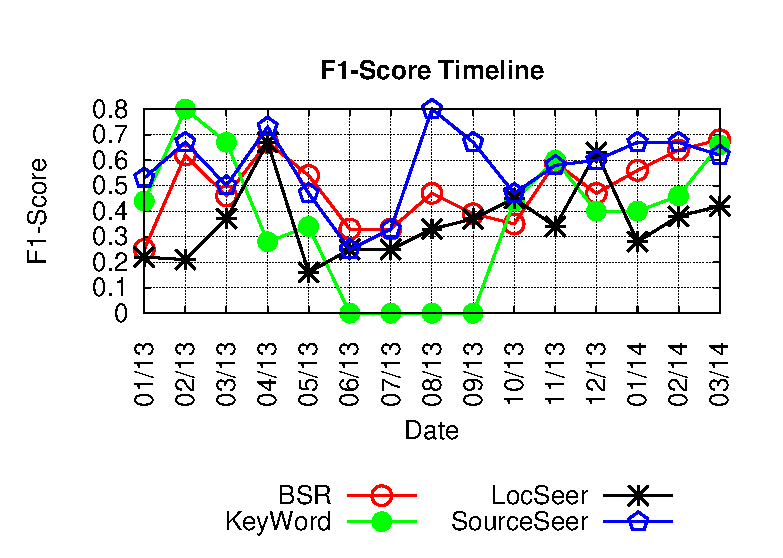
\includegraphics[trim=0 0 0 0, clip,scale=0.44]{fig/f1_timeline.eps} \label{fig:f1_timeline}}
        \subfigure{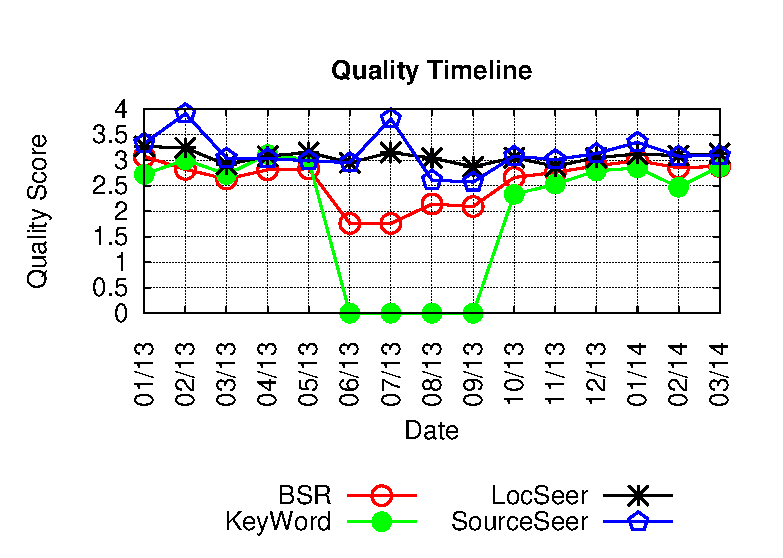
\includegraphics[trim=0 0 0 0, clip,scale=0.44]{fig/quality_timeline.eps} \label{fig:quality_timeline}}
        \subfigure{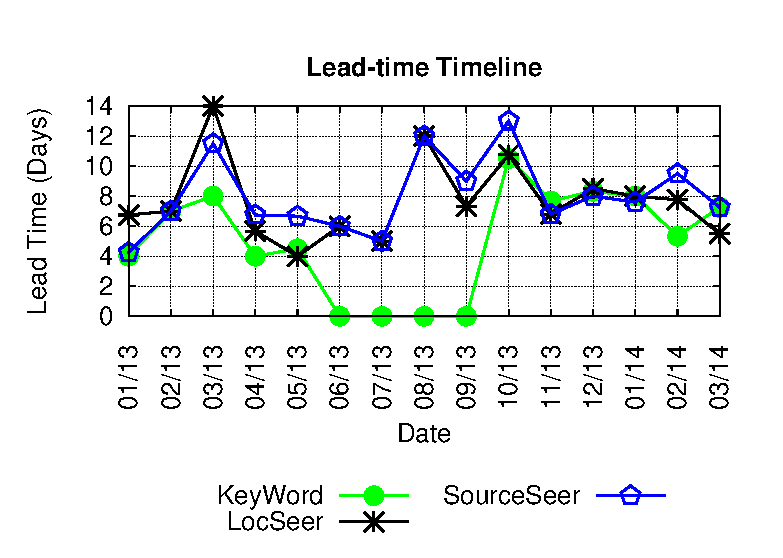
\includegraphics[trim=0 0 0 0, clip,scale=0.44]{fig/lead_timeline.eps} \label{fig:lead_timeline}}
\end{center}
\caption{(a) F1-score timeline (b) quality score timeline for BSR, \keymodel, \locationmodel and \fullmodel on forecasting hantavirus outbreaks. (c) Lead-time timeline for \locationmodel and \fullmodel on predicting hantavirus outbreaks.}
\vspace{-10pt}
\label{fig:perf_timelines}
\end{figure*}


\noindent\textbf{{\em Is the performance gain of {\sf {\bf SourceSeer}}} significant?} To obtain a clearer understanding of \fullmodel's performance gain, we perform the Wilcoxon signed-rank~\cite{Wilcoxon45} test comparing the performance of  BSR with \fullmodel,  \keymodel with \fullmodel and \locationmodel with \fullmodel for precision, recall, and F1-score across all months. The Wilcoxon signed-rank test is a non-parametric statistical hypothesis test used to assess whether the performance differences between two algorithms are statistically significant. In table \Cref{tab:significance} we report the corresponding test statistic scores $W$ and the $z$-scores. We consider a baseline confidence level of $\alpha = .05$. As shown, the performance difference between BSR and \fullmodel is statistically significant for recall and F1 (with \fullmodel outperforming BSR) while the difference for precision is not statistically significant. The exact same behavior was observed for \keymodel and \fullmodel. For \locationmodel and \fullmodel, we see that the performance gain of \fullmodel for precision and F1 is statistically significant while the difference for recall is not. We did not observe significant differences in the performance of \locationmodel and \fullmodel for different threshold values for $k$. 

We further analyze the performance of the four models by comparing the quality score cross all months under consideration. \Cref{fig:quality_timeline} shows the average prediction quality score obtained by each model from January 2013 to March 2014. A higher quality score is an indicator that a model can predict outbreaks correctly at the state and not only at the country level. As shown, both \locationmodel and \fullmodel outperform BSR and \keymodel significantly. This is expected since BSR relies only on past reported events to predict future outbreaks and \keymodel on increased keyword counts, hence, by design both cannot predict outbreaks in states with no reported incidents. Moreover, we observe that \fullmodel obtains higher quality scores for most of the months compared to \locationmodel. This is due to its capability of weighting the predictions of difference sources  based on their accuracy for each specific state.

%\begin{figure}
%\vspace{-10pt}
%\begin{center}
%	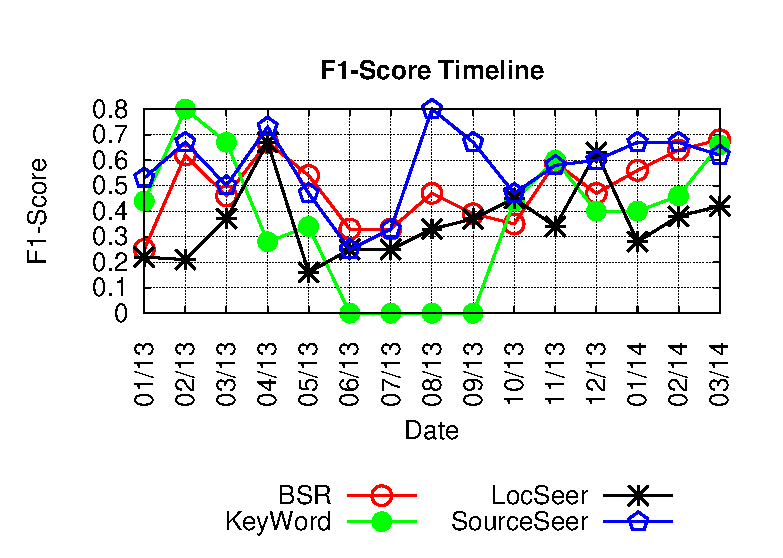
\includegraphics[trim=0 0 0 0, clip,scale=0.5]{fig/f1_timeline.eps}
%\end{center}
%\vspace{-10pt}
%\caption{F1-score timeline for BSR, \keymodel, \locationmodel and \fullmodel on predicting hantavirus outbreaks.}
%\vspace{-10pt}
% \label{fig:f1_timeline}
%\end{figure}

\begin{table*}
\scriptsize \centering
\caption{Wilcoxon signed-rank statistical significance test on \fullmodel's performance gain. $H_0$: The median performance difference between the pairs is zero. Reject $H_0$: $\|z\| \geq 1.645$ or $W \geq 15$ when $z$ not applicable. Baseline confidence level of $\alpha =.05$.}
\begin{tabular}{|c|c|c|c|c|} 
\hline
{\bf Metric} & {\bf Score} & {\bf BSR v.s. \fullmodel} & {\bf \locationmodel v.s. \fullmodel} & {\bf \keymodel v.s. \fullmodel} \\ \hline
\multirow{2}{*}{{\bf Prec.}} & W & -51 & 81 & 36\\
& z & -1.463 & 2.966 & 1.349\\ \hline
\multirow{2}{*}{{\bf Rec.}} & W & 114 & 3&76\\
& z & 3.223 & -&2.961\\ \hline
\multirow{2}{*}{{\bf F1}} & W & 61 & 101&100\\
& z & 1.899 & 3.154&2.825\\ \hline
\end{tabular}
\label{tab:significance}
\end{table*}

\noindent\textbf{{\em What is the lead-time gain of {\sf {\bf SourceSeer}}?}} Finally, we analyze the average lead-time of \keymodel, \locationmodel and \fullmodel to examine if the proposed models can forecast outbreaks in a timely manner. \Cref{fig:lead_timeline} shows the lead-time timeline of the three models from January 2013 to March 2014. We observe that both models have a significant lead-time advantage when compared against  the mention of the outbreak in news sources and also outperform \keymodel.

%\begin{figure}
%\vspace{-10pt}
%\begin{center}
%	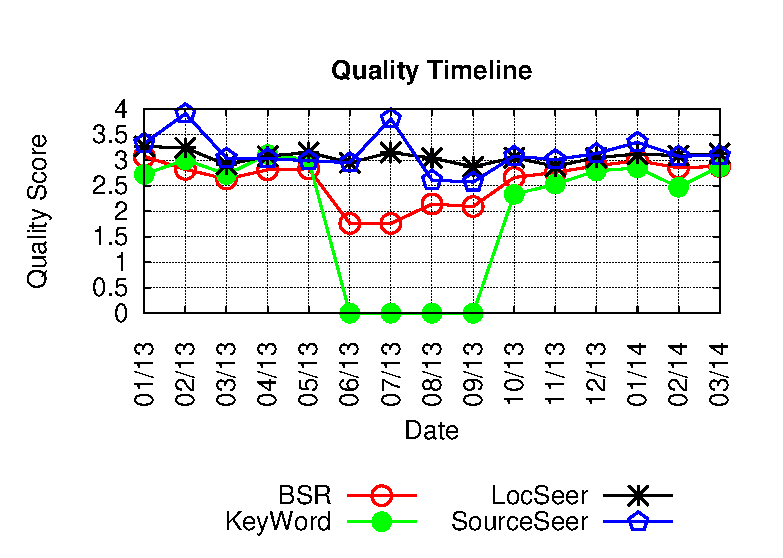
\includegraphics[trim=0 0 0 0, clip,scale=0.5]{fig/quality_timeline.eps}
%\end{center}
%\vspace{-10pt}
%\caption{Quality score timeline for BSR, \keymodel, \locationmodel and \fullmodel on predicting hantavirus outbreaks.}
%\vspace{-10pt}
% \label{fig:quality_timeline}
%\end{figure}

\subsection{Discussion}
From our experiments we see that \fullmodel can effectively discover rare-disease topics and their spatio-temporal patterns. We also observed that exploiting the different authoritativeness levels of news sources enables us to forecast outbreaks more accurately even when no outbreaks were reported in the past. Finally, \fullmodel can forecast outbreaks ahead of news media with an average lead-time of 8 days.

%\subsection{Analyzing Data Sources}
%Next, we examine the accuracy of the data source for the four countries under consideration. The source accuracies are used to determine the confidence of each outbreak prediction and hence are crucial for the performance of \fullmodel. \Cref{fig:src_char} shows the source accuracy histograms for Chile, Argentina, Brazil and Uruguay. As shown, in Uruguay, Argentina and Brazil, most of the sources exhibit high accuracy. On the other hand the majority of news sources for Chile have a low accuracy. The reason is that due to the increased number of hantavirus incidents in Chile, there is a constant flow of related news articles leading to false outbreak predictions for many sources. However, there are several sources that exhibit high accuracy. As shown before, \fullmodel was able to exploit this fact and limit the number of falsely predicted outbreaks.
%
%\begin{figure*}[ht]
%\begin{center}
%        \subfigure{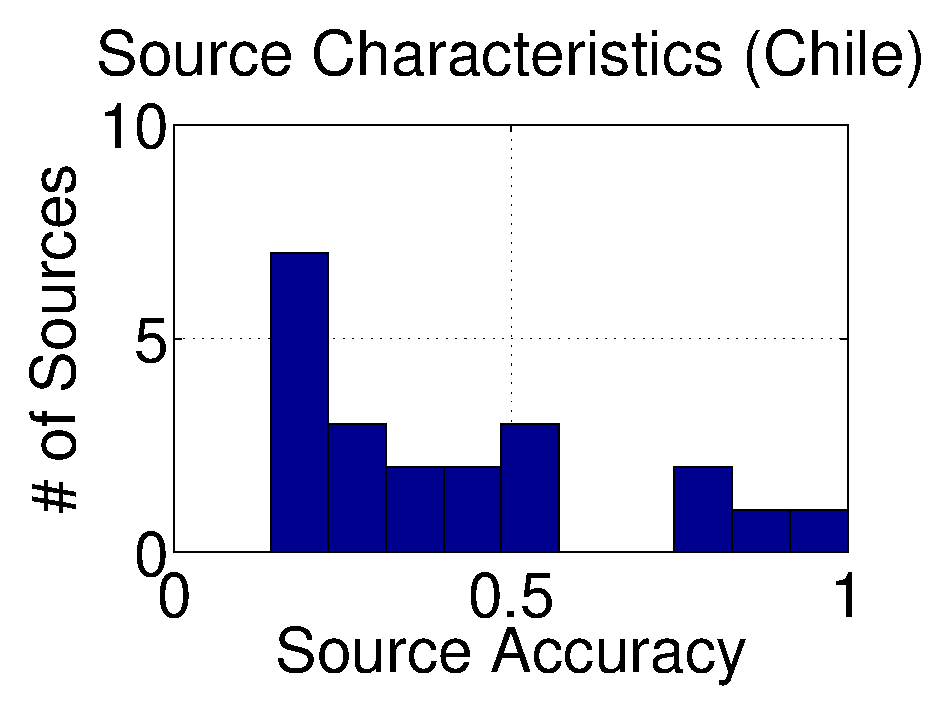
\includegraphics[clip,scale=0.25]{fig/chile_src.eps}  \label{fig:chile_src}}
%        \subfigure{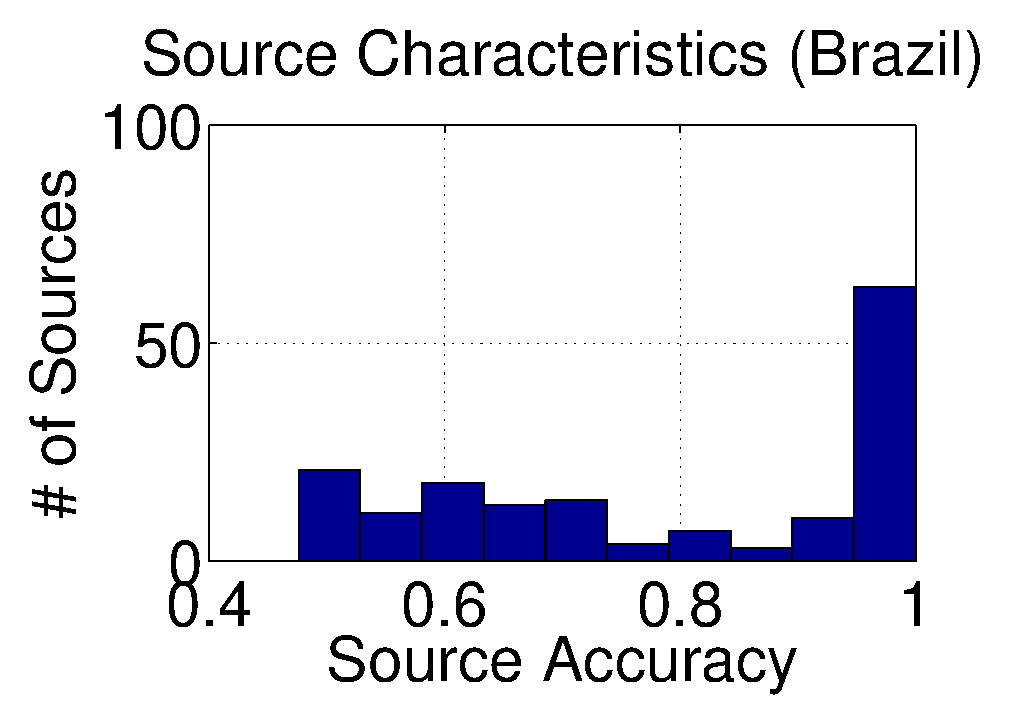
\includegraphics[clip,scale=0.25]{fig/brazil_src.eps} \label{fig:brazil_src}}
%        \subfigure{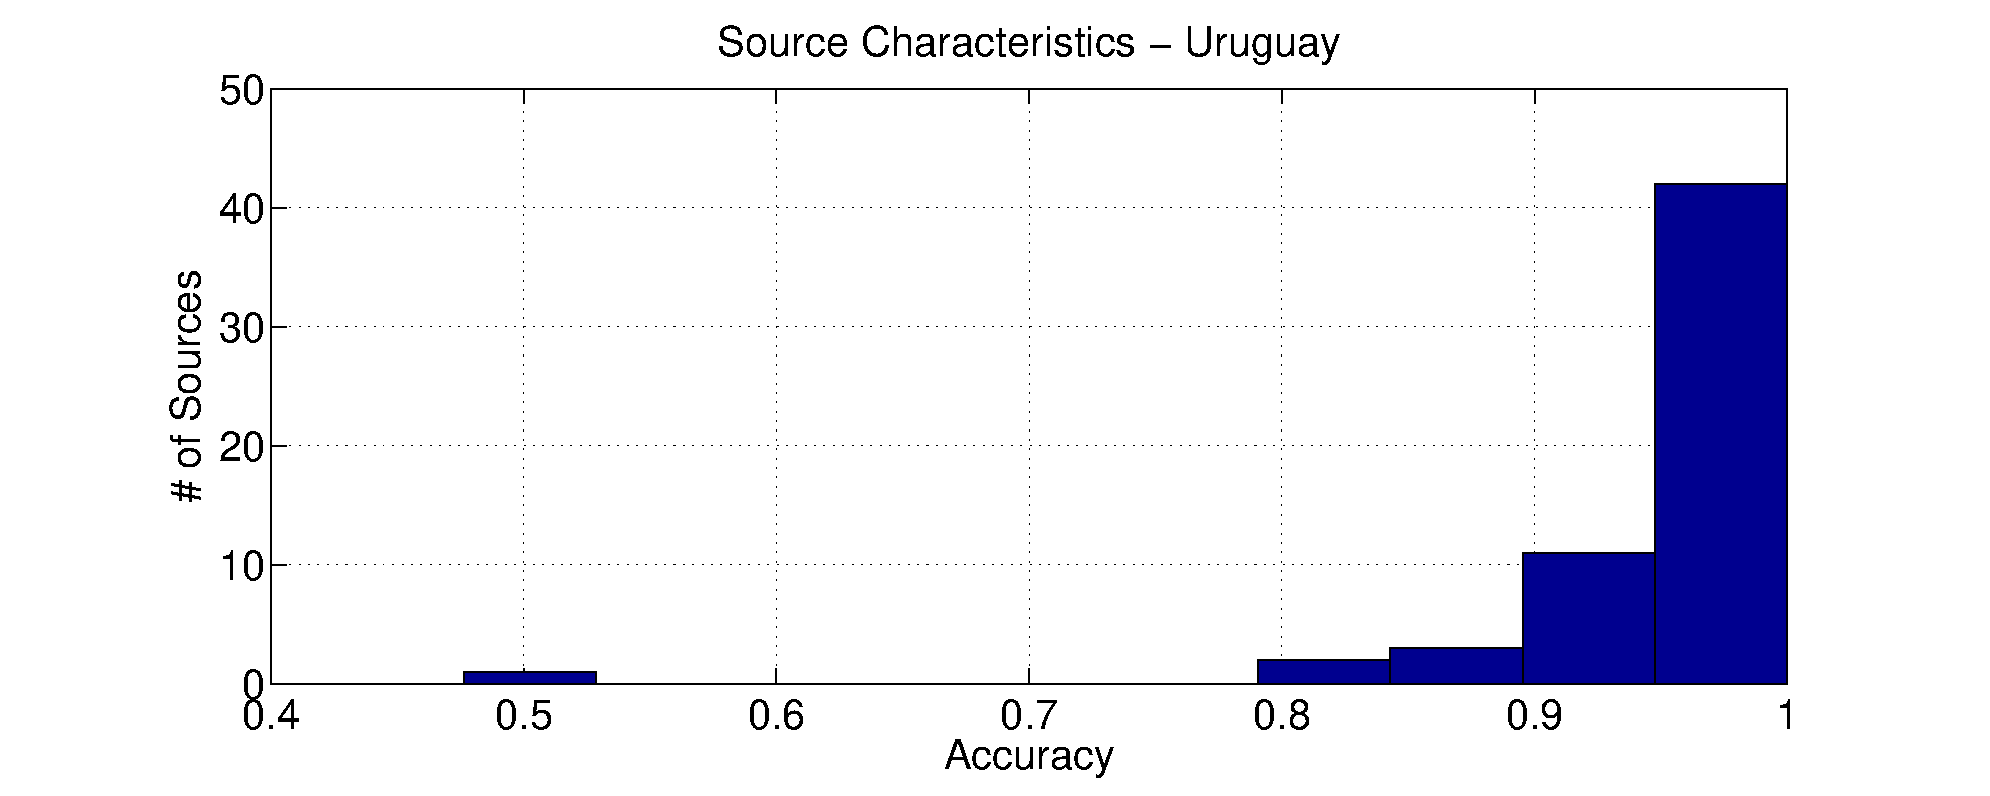
\includegraphics[clip,scale=0.25]{fig/argentina_src.eps} \label{fig:arg_src}}
%        \subfigure{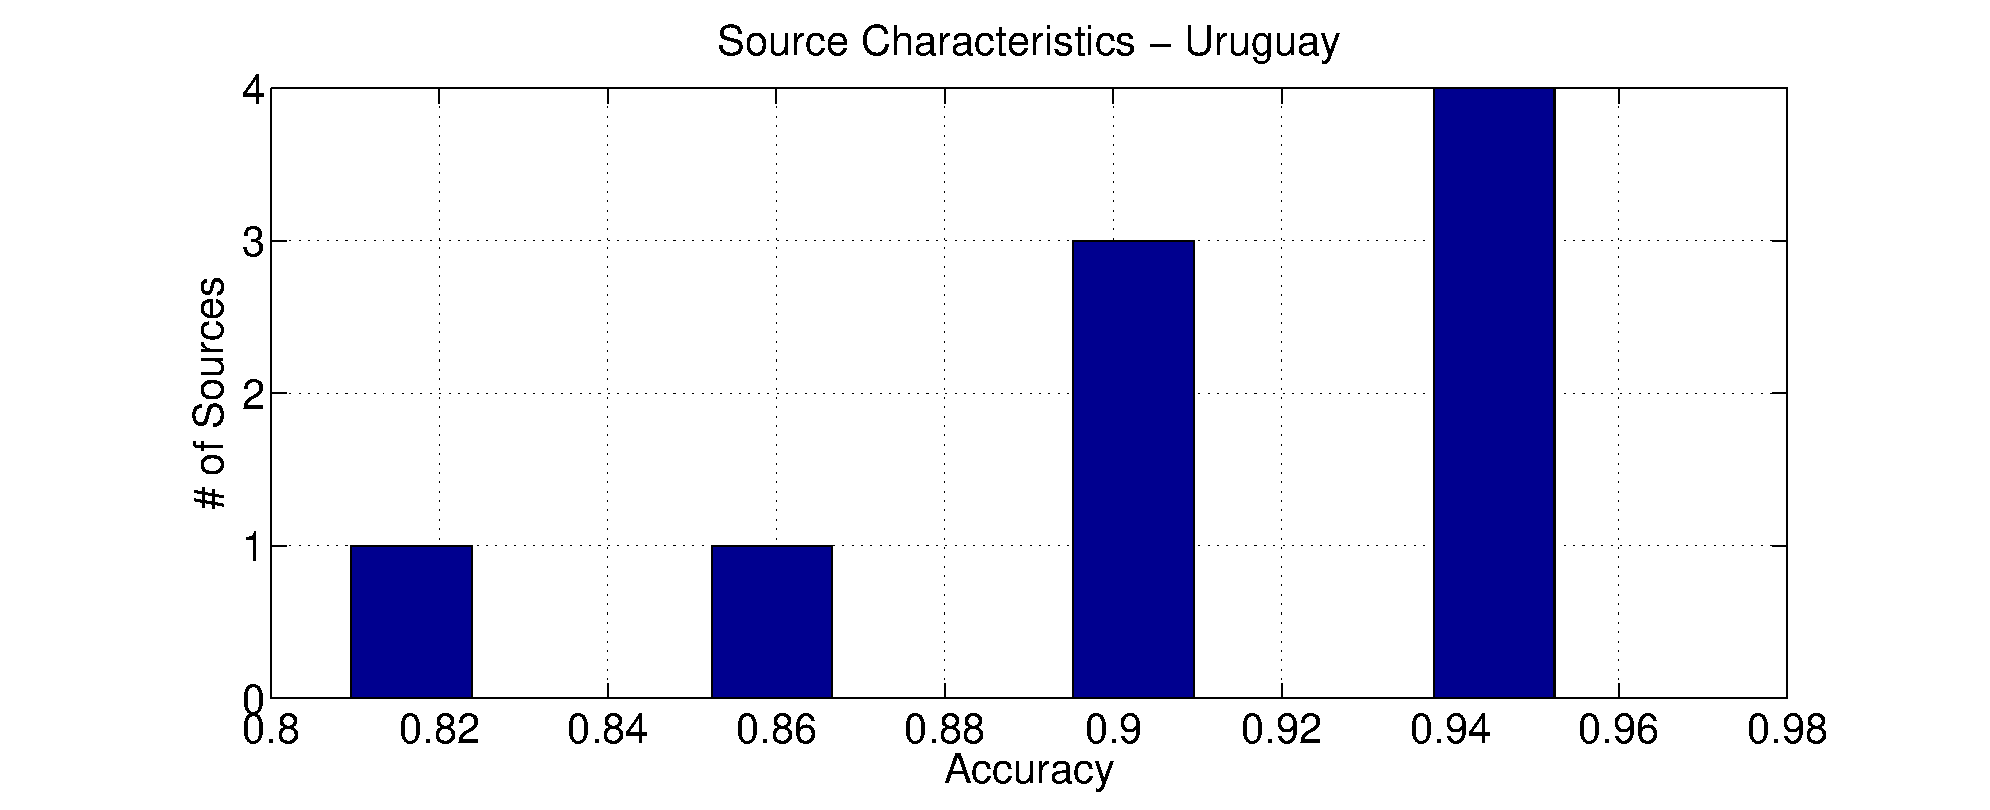
\includegraphics[clip,scale=0.25]{fig/uruguay_src.eps}  \label{fig:urug_src}}        
%\end{center}
%\caption{Source accuracy histograms for Chile, Brazil, Argentina and Uruguay.}
%\label{fig:src_char}
%\end{figure*}


%\begin{figure*}[ht]
%\begin{center}
%        \subfigure{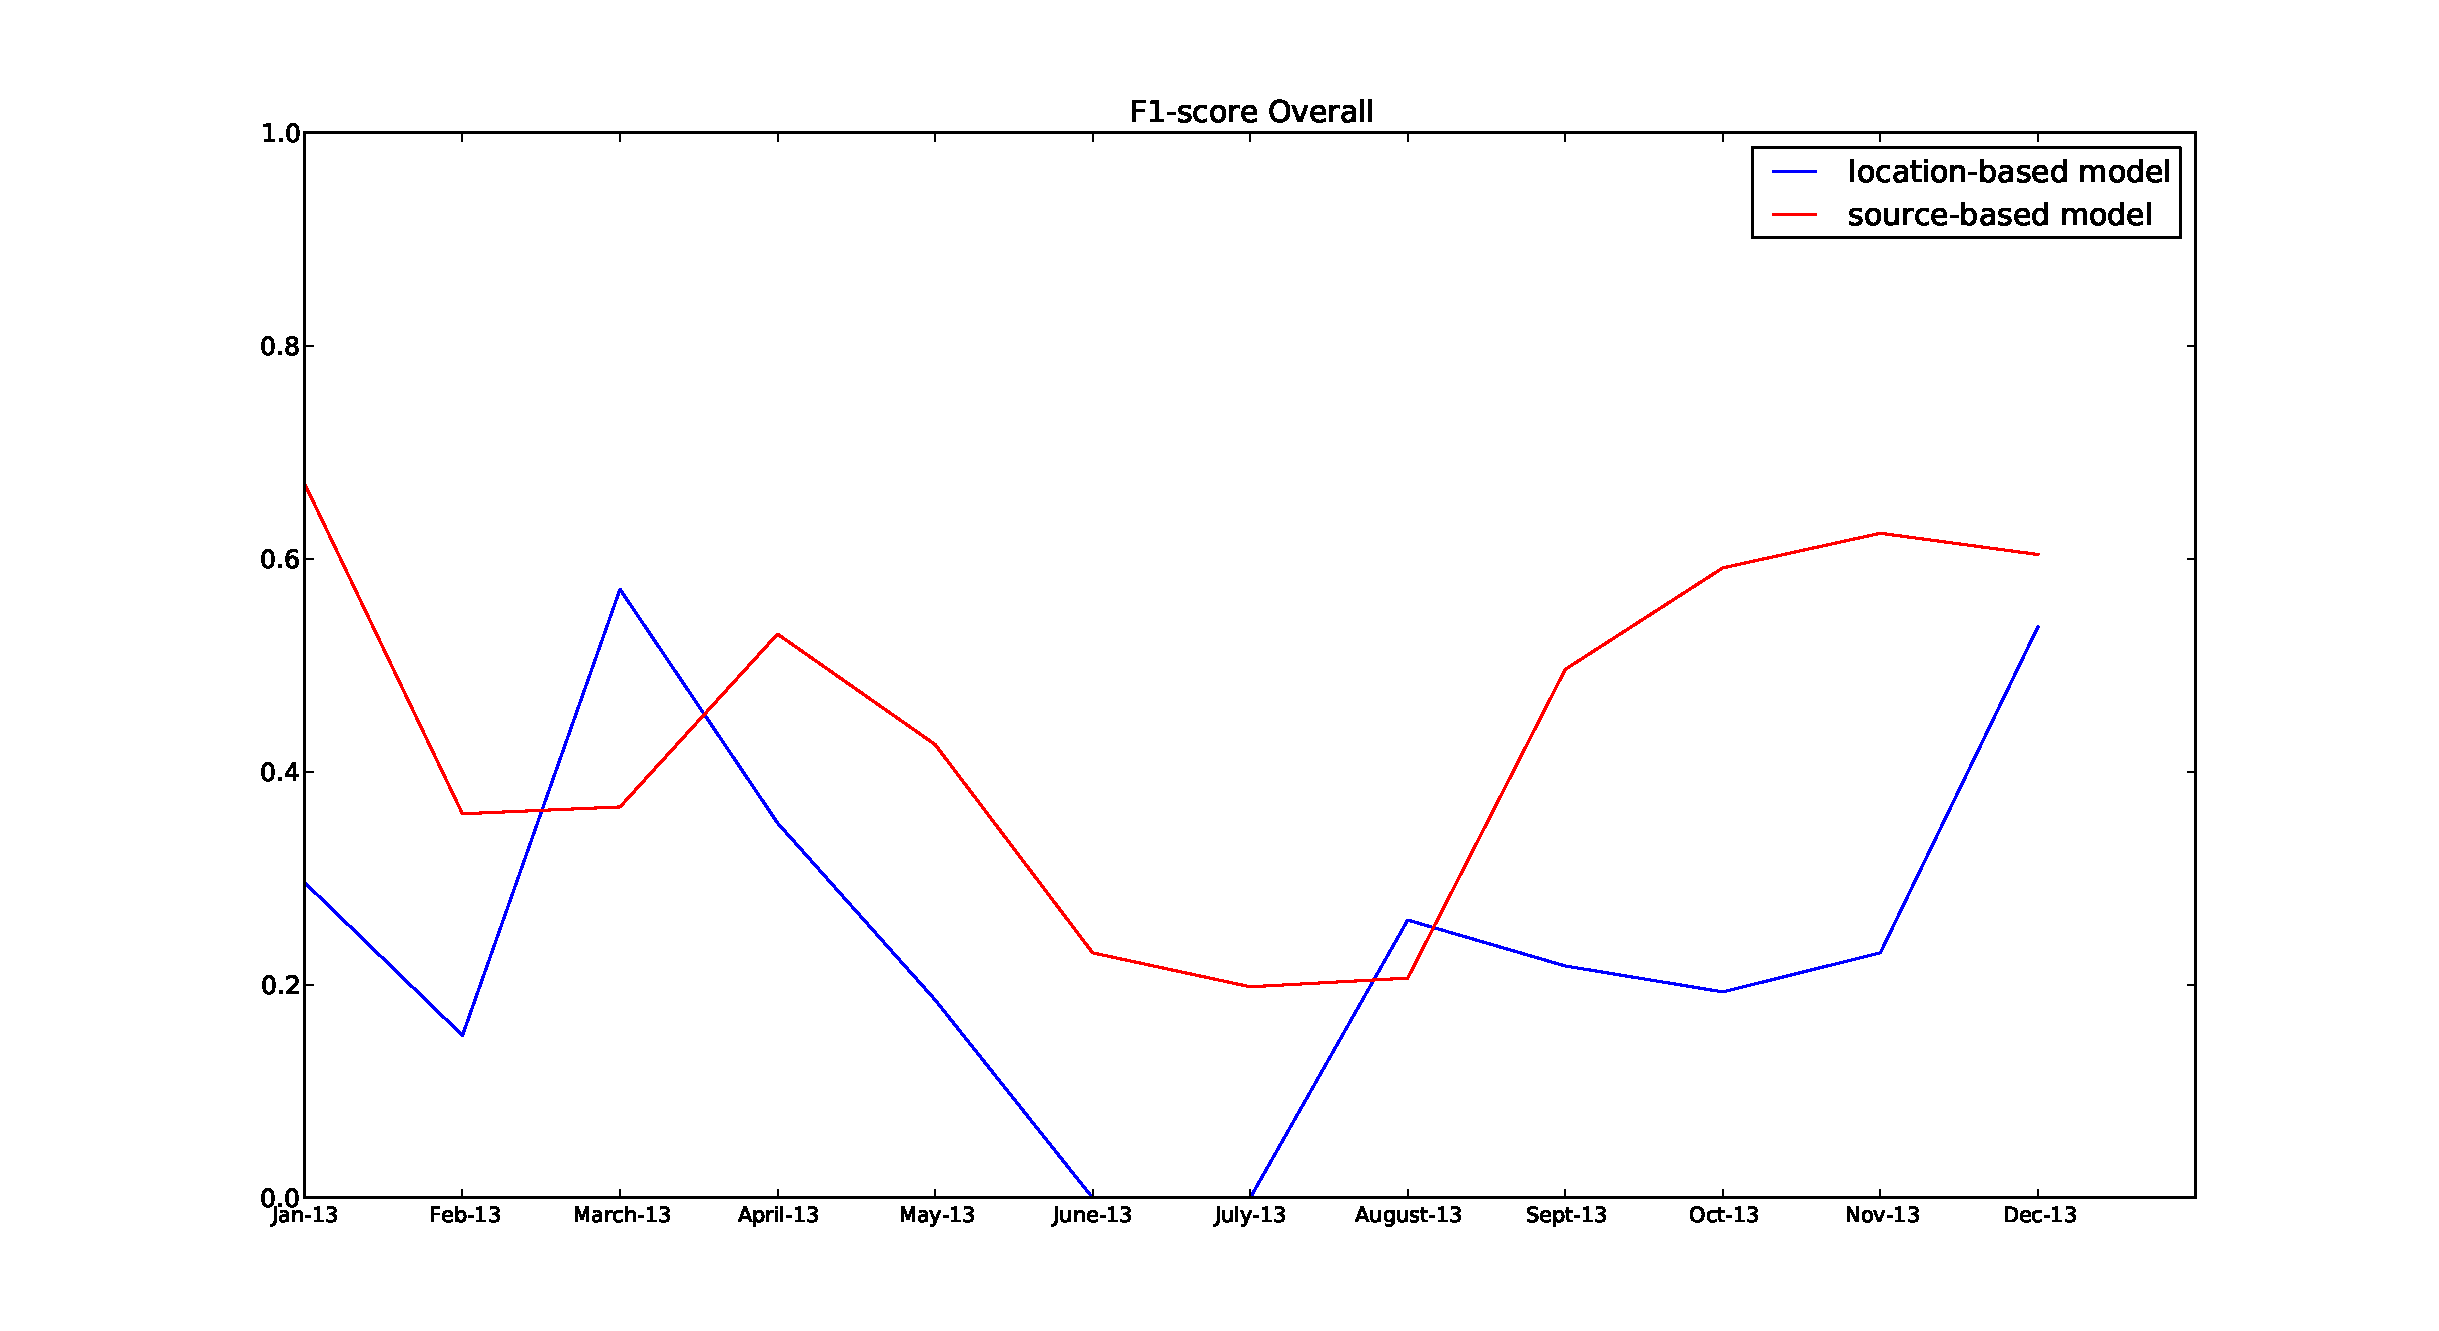
\includegraphics[scale=0.13]{figures/F1-score-overall.pdf}\label{fig:F1-score}}
%        \subfigure{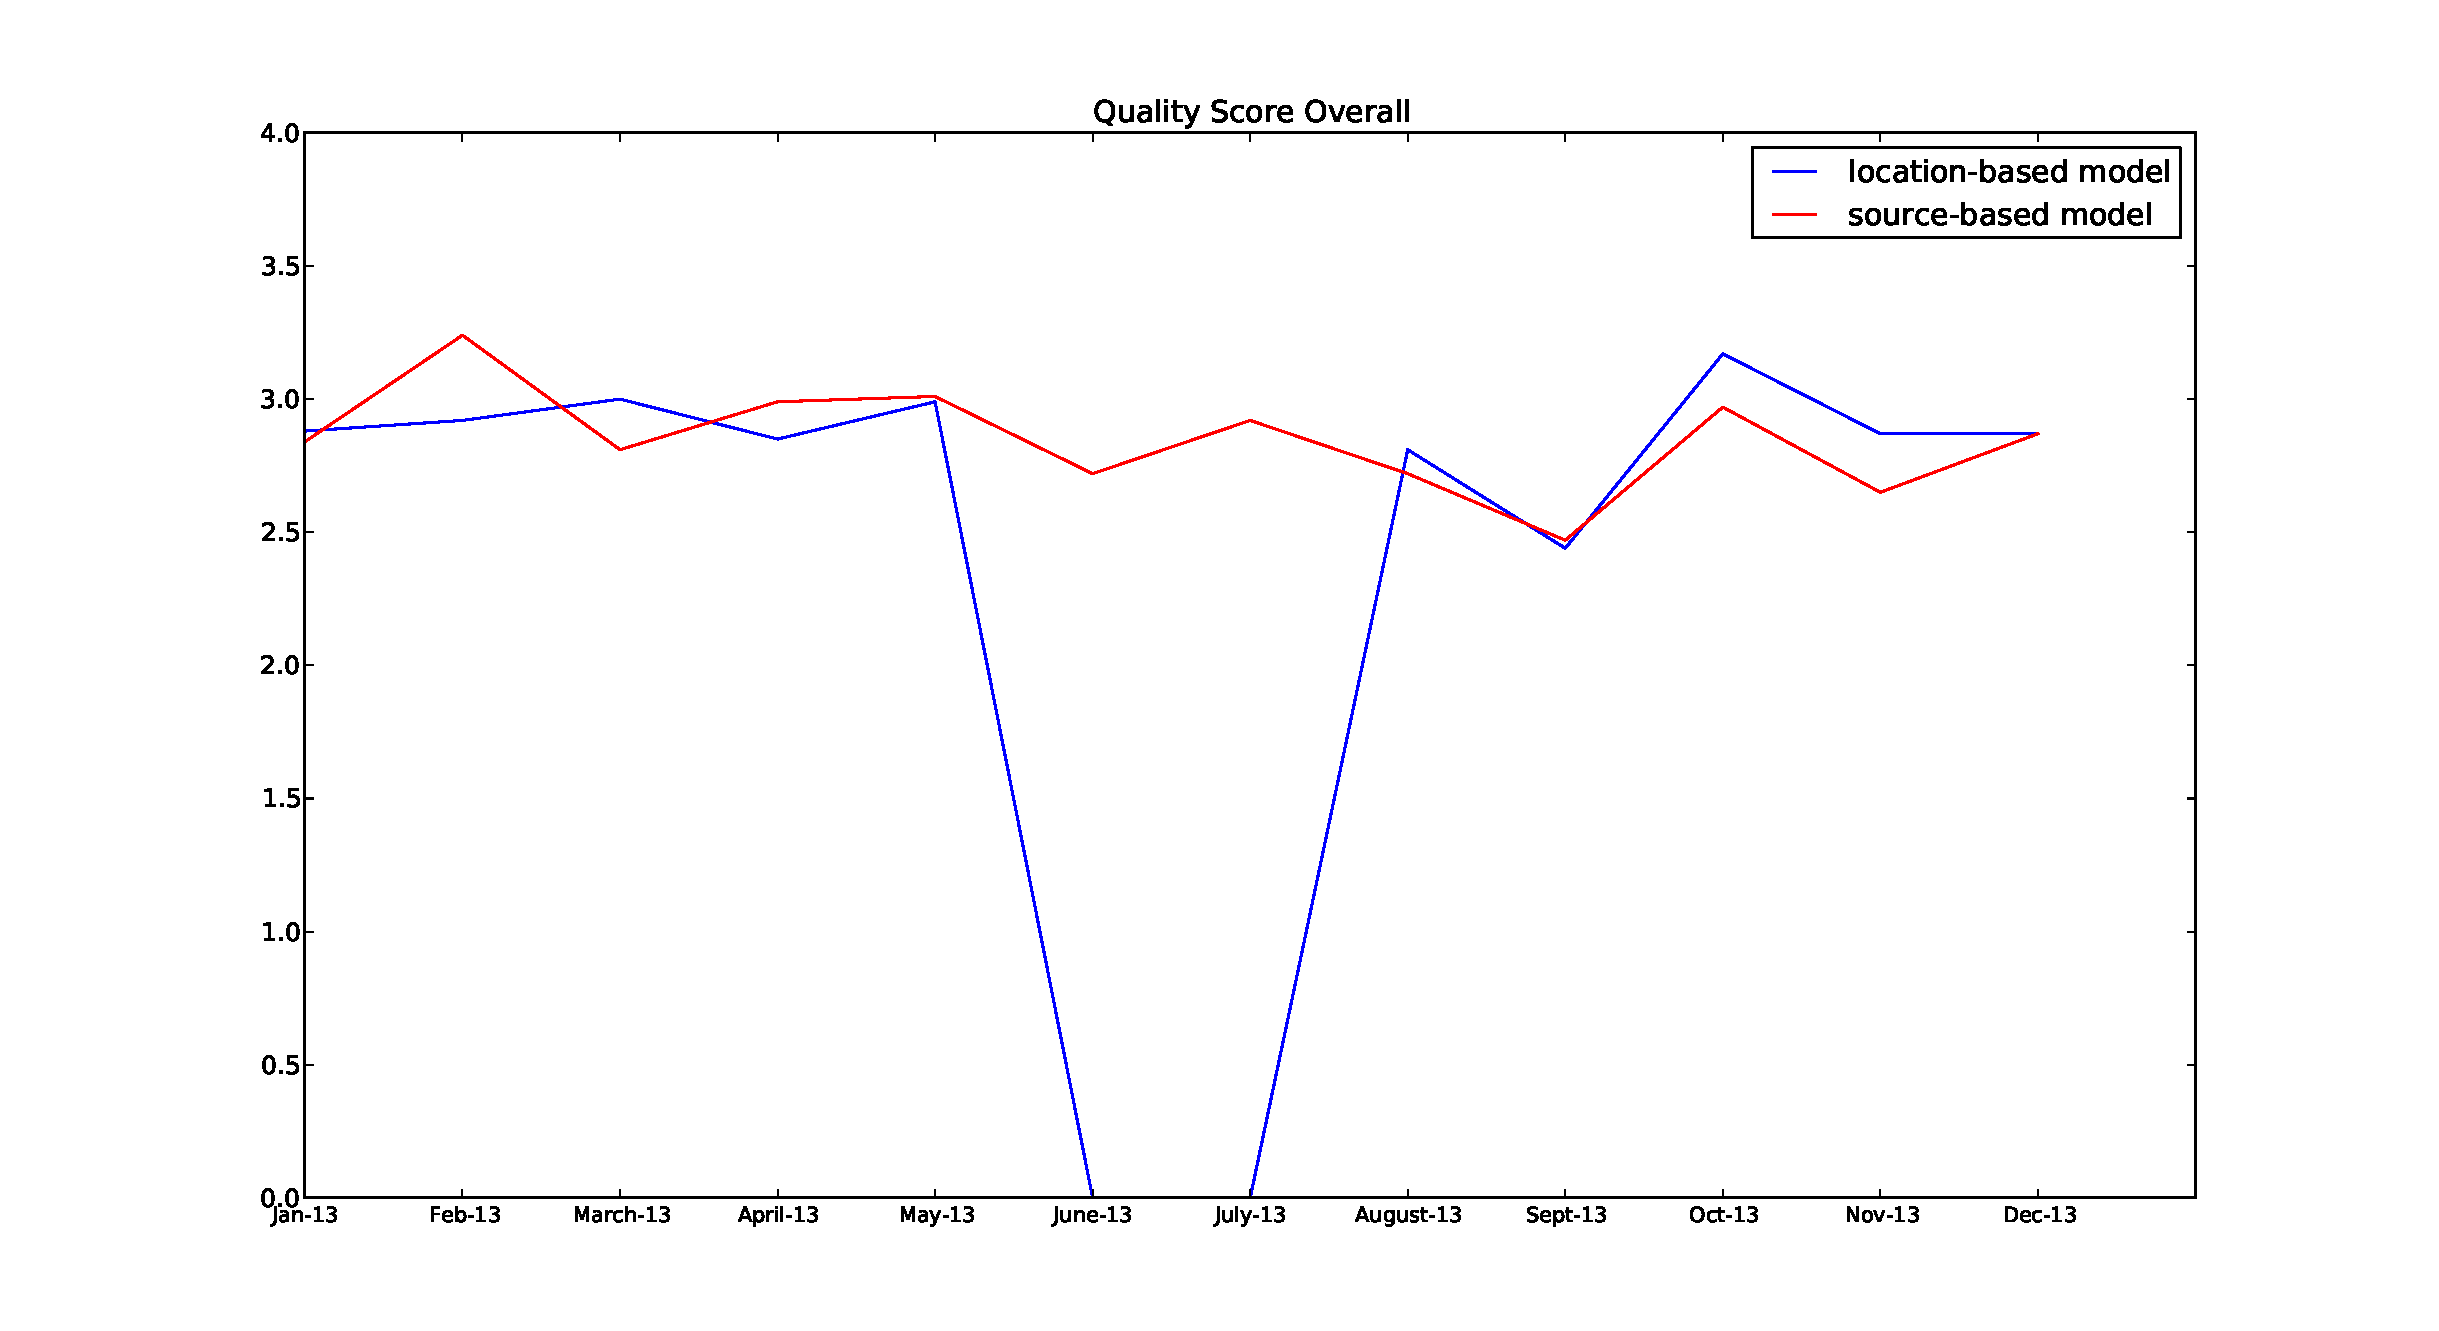
\includegraphics[scale=0.13]{figures/QS_overall.pdf}\label{fig:QS}}
%        \subfigure{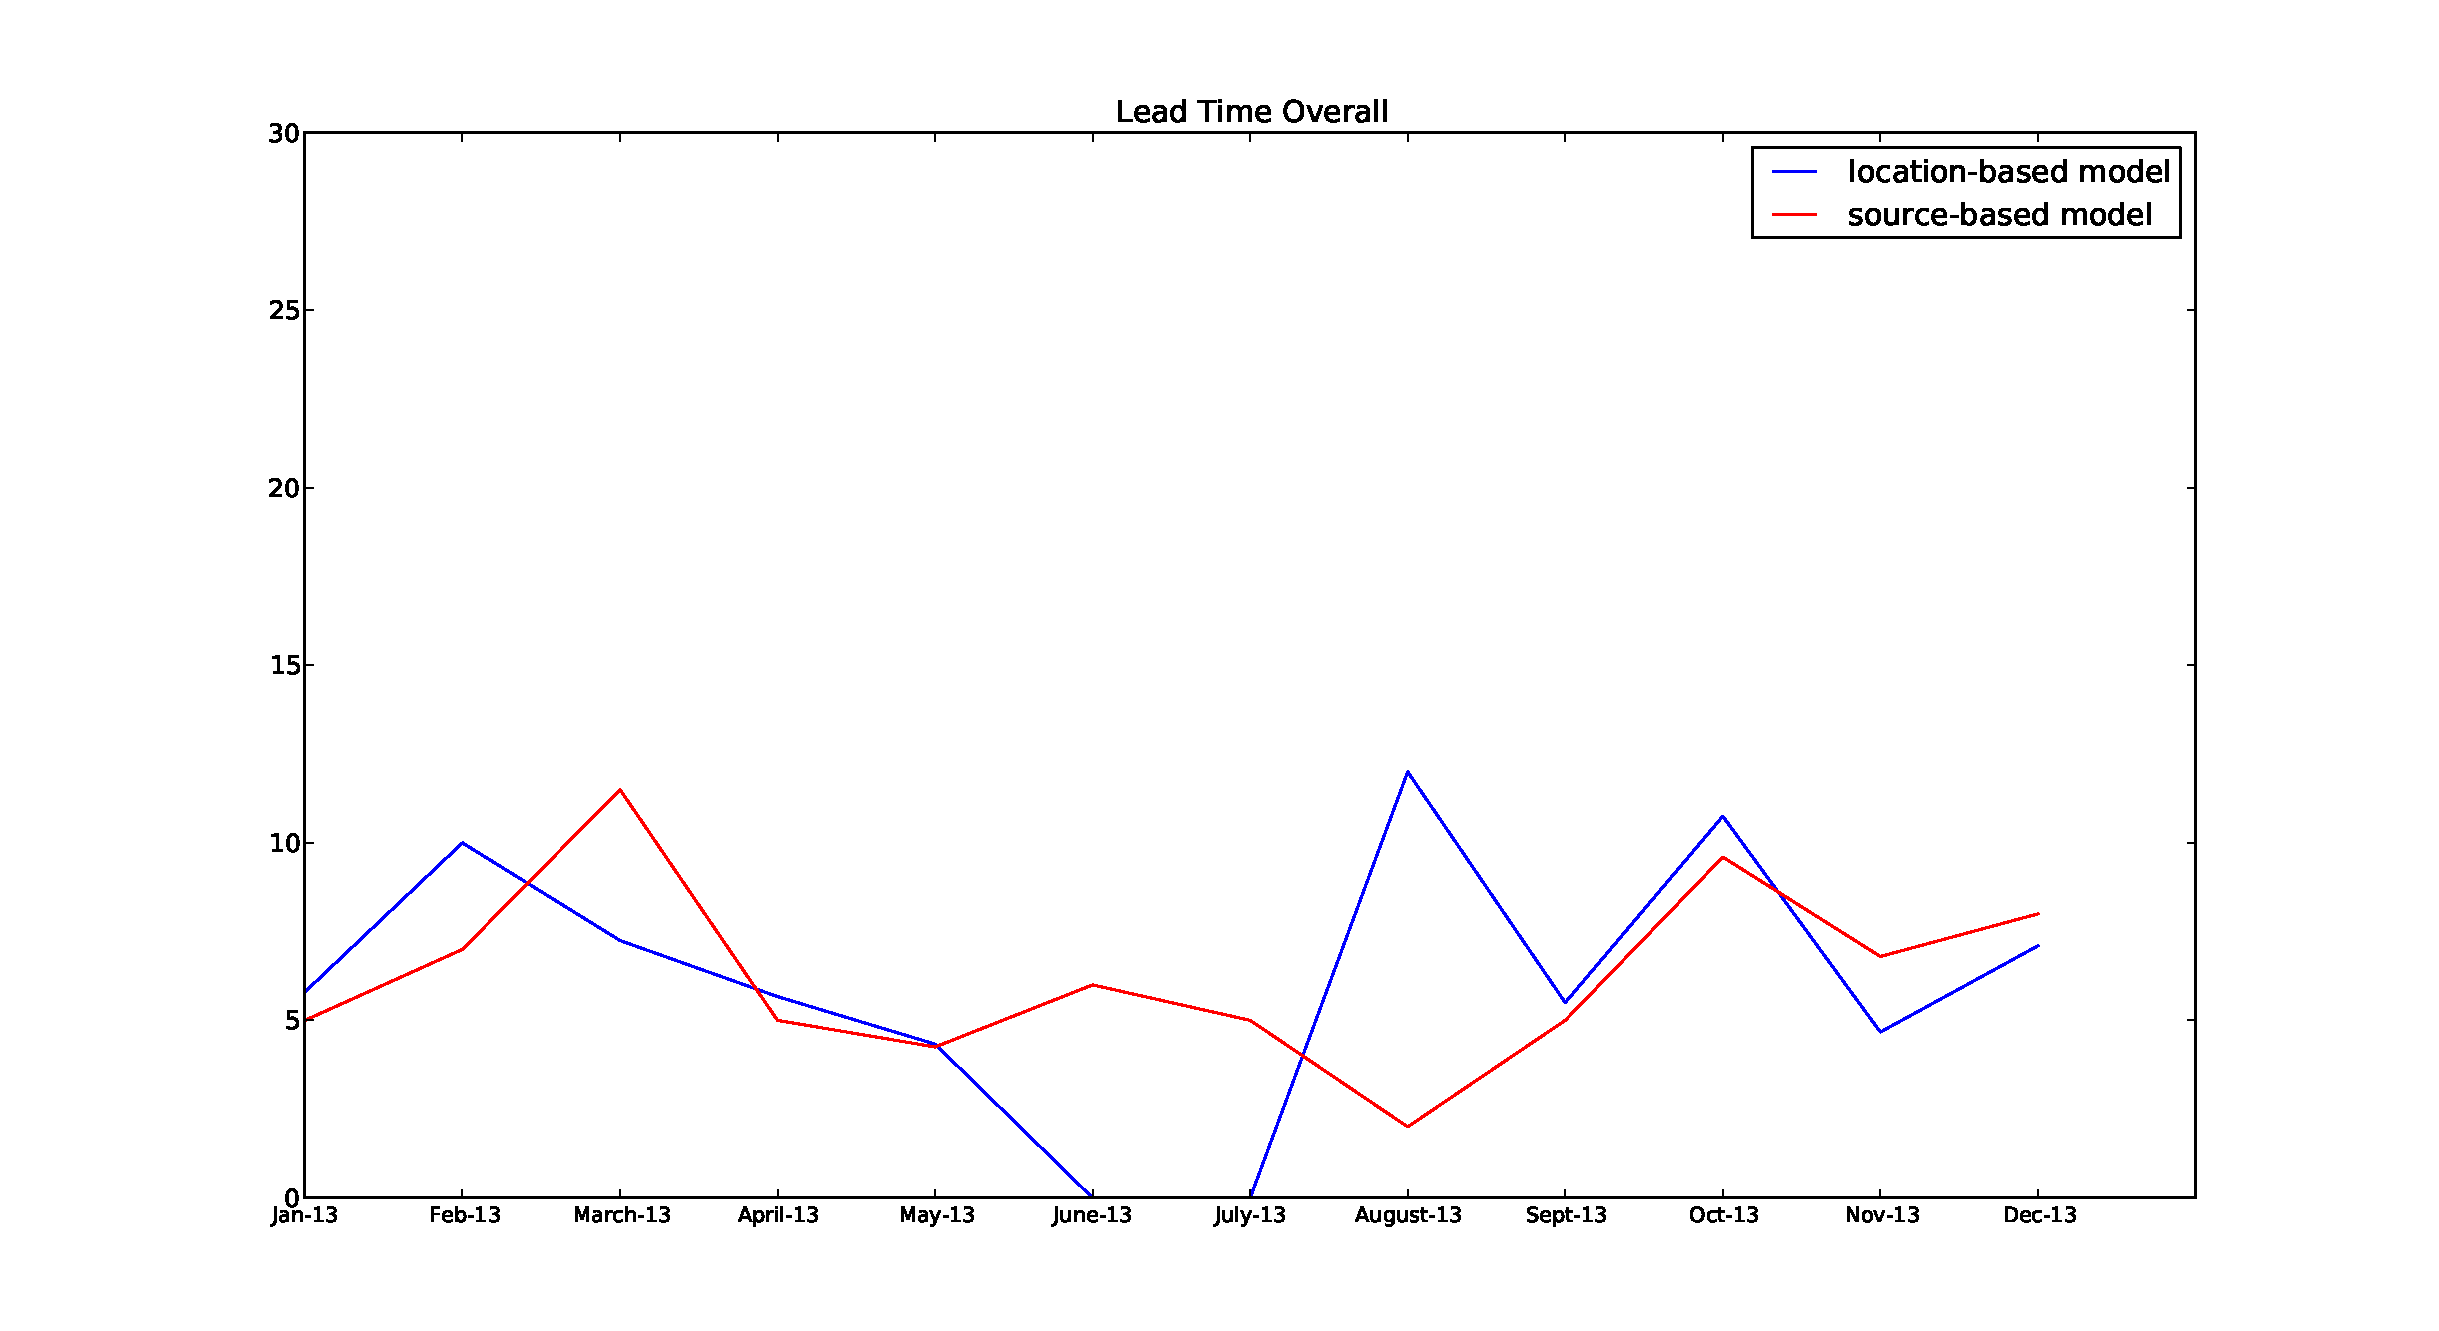
\includegraphics[scale=0.13]{figures/Lead_time_overall.pdf}\label{fig:LT}}
%\end{center}
%\caption{Comparison plots of S-STAT and L-STAT in terms of (a)
%F1-score,(b) Quality Score and (c) Lead Time}
%\label{fig:evaluation_metric}
%\end{figure*}
%
\section{Related Work}
\label{sec:related_work}
Much of the work in the topic models literature has focused on identifying either spatial or temporal trends for the discovered topics. To the best of our knowledge most models focus on the temporal or spatial trends in isolation and do not analyze both types of trends jointly.  Moreover, none of the models considers the accuracy of different data sources analyzed to predict outbreaks.

%\begin{figure}[h]
%\vspace{-10pt}
%\begin{center}
%	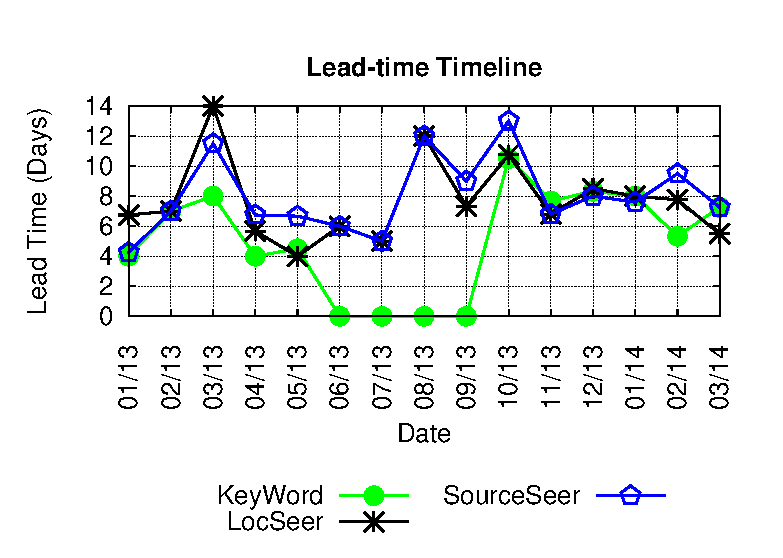
\includegraphics[trim=0 0 0 0, clip,scale=0.5]{fig/lead_timeline.eps}
%\end{center}
%\vspace{-20pt}
%\caption{Lead-time timeline for \locationmodel and \fullmodel on predicting hantavirus outbreaks.}
% \label{fig:lead_timeline}
% \vspace{-15pt}
%\end{figure}

A number of methods have been proposed for analyzing the time evolution of topics in document collections, such as the topics over time (TOT) model~\cite{wang:2006}, the dynamic topic model (DTM)~\cite{blei:2006}, and TriMine model~\cite{matsubara:2012}.  More precisely, TOT handles time-windows of fixed size and uses a Beta distribution to model the evolution of a topic over time. DTM  also focuses on a time-window of fixed size but uses Kalman filters to align topics with different time points. Finally, TriMine is able to analyze windows of variate size and unlike TOT and DTM is able to find cyclic time patterns with different timescales, which enables predicting future events. While TOT and DTM focus on the dimension of time alone, TriMine can associate the generation of different modalities with topics, however is agnostic to correlations across the different modalities.

A different line of work~\cite{wang:2007} focuses on discovering spatial patterns jointly with the word co-occurrences. In particular, the authors introduced the Spatial Latent Dirichlet Allocation (SLDA), which better encodes spatial structure among words. While the model focuses on computer vision applications where documents are comprised by visual words the proposed techniques can be trivially extended to regular text documents. A similar approach was introduced by Ramage et al.~\cite{ramage:2009} for labeled documents where the labels can correspond to multiple modalities, i.e., locations as well.

Finally, although previous approaches~\cite{paul:11, sadilek:2012, rider:2013} have considered the use of topic models for forecasting disease outbreaks, they mainly focus on common diseases, like influenza, for which large amounts of publicly available data or specialized medical records are available. 

\section{Conclusions}
\label{sec:conclusion}
We studied the problem of rare disease outbreak prediction when analyzing dynamic news sources providing an evolving corpus of news articles. We introduced \fullmodel, a framework that combines spatio-temporal topic models with source-based anomaly detection techniques for forecasting rare disease outbreaks at fine spatial granularity by considering the accuracy of each individual news source. Experimental results show the effectiveness of our proposed framework and illustrate how taking the accuracy of data sources into account leads to higher quality predictions.

\begin{thebibliography}{10}

\bibitem{probmed}
International society for infectious diseases.
\newblock \url{www.promedmail.org/}.

\bibitem{arora:2012}
S.~Arora, E.~Hazan, and S.~Kale.
\newblock The multiplicative weights update method: a meta-algorithm and
  applications.
\newblock {\em Theory of Computing}, 8(1), 2012.

\bibitem{blei:2006}
D.~M. Blei and J.~D. Lafferty.
\newblock Dynamic topic models.
\newblock ICML, 2006.

\bibitem{blei:2003}
D.~M. Blei, A.~Y. Ng, and M.~I. Jordan.
\newblock Latent dirichlet allocation.
\newblock {\em JMLR}, 3, 2003.

\bibitem{brownstein:2008}
J.~S. Brownstein, C.~C. Freifeld, B.~Y. Reis, and K.~D. Mandl.
\newblock {Surveillance Sans Fronti\`{e}res: Internet-Based Emerging Infectious
  Disease Intelligence and the HealthMap Project}.
\newblock {\em PLoS Medicine}, 5(7), 2008.

\bibitem{corley:10}
C.~Corley, D.~Cook, A.~Mikler, and K.~Singh.
\newblock Text and structural data mining of influenza mentions in web and
  social media.
\newblock {\em IJERPH}, 7(2), 2010.

\bibitem{culotta:2010}
A.~Culotta.
\newblock Towards detecting influenza epidemics by analyzing twitter messages.
\newblock SOMA, 2010.

\bibitem{healthmap}
C.~C. Freifeld, K.~D. Mandl, B.~Y. Reis, and J.~S. Brownstein.
\newblock {HealthMap: Global Infectious Disease Monitoring through Automated
  Classification and Visualization of Internet Media Reports}.
\newblock {\em JAMIA}, 15, 2008.

\bibitem{ginsberg:09}
J.~Ginsberg, M.~H. Mohebbi, R.~S. Patel, L.~Brammer, M.~S. Smolinski, and
  L.~Brilliant.
\newblock {Detecting influenza epidemics using search engine query data}.
\newblock {\em Nature}, 457, 2009.

\bibitem{heller:03}
K.~A. Heller, K.~M. Svore, A.~D. Keromytis, and S.~J. Stolfo.
\newblock One class support vector machines for detecting anomalous windows
  registry accesses.
\newblock In {\em Data Mining for Computer Security}, 2003.

\bibitem{jonsson:10}
C.~B. Jonsson, L.~T.~M. Figueiredo, and O.~Vapalahti.
\newblock A global perspective on hantavirus ecology, epidemiology and disease.
\newblock {\em Clinical Microbiology Review}, 23(2), 2010.

\bibitem{khan:13}
S.~S. Khan and M.~G. Madden.
\newblock One-class classification: Taxonomy of study and review of techniques.
\newblock {\em CoRR}, abs/1312.0049, 2013.

\bibitem{linge:09}
J.~P. Linge, R.~Steinberger, T.~P. Weber, R.~Yangarber, and E.~van~der Goot.
\newblock Internet surveillance systems for early alerting of health threats.
\newblock {\em Eurosurveillance}, 14(13), 2009.

\bibitem{manevitz:2002}
L.~M. Manevitz and M.~Yousef.
\newblock One-class svms for document classification.
\newblock {\em JMLR}, 2, 2002.

\bibitem{matsubara:2012}
Y.~Matsubara, Y.~Sakurai, C.~Faloutsos, T.~Iwata, and M.~Yoshikawa.
\newblock Fast mining and forecasting of complex time-stamped events.
\newblock KDD, 2012.

\bibitem{parker:13}
J.~Parker, Y.~Wei, A.~Yates, O.~Frieder, and N.~Goharian.
\newblock A framework for detecting public health trends with twitter.
\newblock ASONAM, 2013.

\bibitem{paul:11}
M.~Paul and M.~Dredze.
\newblock You are what you tweet: Analyzing twitter for public health, 2011.

\bibitem{ramage:2009}
D.~Ramage, D.~Hall, R.~Nallapati, and C.~D. Manning.
\newblock Labeled lda: A supervised topic model for credit attribution in
  multi-labeled corpora.
\newblock EMNLP, 2009.

\bibitem{rider:2013}
A.~K. Rider and N.~V. Chawla.
\newblock An ensemble topic model for sharing healthcare data and predicting
  disease risk.
\newblock BCB, 2013.

\bibitem{sadilek:2012}
A.~Sadilek, H.~A. Kautz, and V.~Silenzio.
\newblock Predicting disease transmission from geo-tagged micro-blog data.
\newblock AAAI, 2012.

\bibitem{schoelkopf:99}
B.~Schoelkopf, J.~C. Platt, J.~Shawe-Taylor, A.~J. Smola, and R.~C. Williamson.
\newblock Estimating the support of a high-dimensional distribution.
\newblock {\em Neural Computation}, 13, 1999.

\bibitem{steinwart:05}
I.~Steinwart, D.~Hush, and C.~Scovel.
\newblock A classification framework for anomaly detection.
\newblock {\em JMLR}, 6, 2005.

\bibitem{strehl:2000}
A.~Strehl, E.~Strehl, J.~Ghosh, and R.~Mooney.
\newblock Impact of similarity measures on web-page clustering.
\newblock In {\em AI for Web Search}, AAAI, 2000.

\bibitem{wang:2007}
X.~Wang and E.~Grimson.
\newblock Spatial latent dirichlet allocation.
\newblock NIPS, 2007.

\bibitem{wang:2006}
X.~Wang and A.~McCallum.
\newblock Topics over time: A non-markov continuous-time model of topical
  trends.
\newblock KDD, 2006.

\bibitem{Wilcoxon45}
F.~Wilcoxon.
\newblock {Individual Comparisons by Ranking Methods}.
\newblock {\em Biometrics Bulletin}, 1(6), 1945.

\bibitem{wong:02}
W.-K. Wong, A.~Moore, G.~Cooper, and M.~Wagner.
\newblock Rule-based anomaly pattern detection for detecting disease outbreaks.
\newblock AAAI, 2002.

\bibitem{wong:03}
W.-K. Wong, A.~Moore, G.~Cooper, and M.~Wagner.
\newblock Bayesian network anomaly pattern detection for disease outbreaks.
\newblock ICML, 2003.
\end{thebibliography}


\clearpage
\appendix
\noindent\textbf{Appendix}

\section{Gibbs Sampling for \model}
\label{sec:gibbs}
In this section we first provide a Gibbs sampling algorithm for learning the parameters of the topic model introduced in \Cref{sec:model}. Before we proceed with the actual algorithm we present the joint distribution corresponding to the topic model. We have the following:
\begin{align}
&\Pr(\w,\tim,\loc,\z,{\bf \phi},{\bf \theta},{\bf \xi};\alpha,\beta,\gamma) =  \nonumber \\
&=\prod_{z = 1}^{K}\Pr(\phi_z;\beta)\Pr(\xi_z;\gamma) \prod_{l = 1}^{L}\Pr(\theta_l;\alpha) \nonumber \\
& \cdot \prod_{s = 1}^{S}\prod_{i = 1}^{N_s} \Pr(z_{si}|l_{si},\theta_l)\Pr(w_{si}|\phi_{z_{si}})\Pr(t_{si}|\xi_{z_{si}}) \nonumber
\end{align}
Next, we marginalize over all ${\bf \phi}$, ${\bf \xi}$ and ${\bf \theta}$. We have:
{\scriptsize
\begin{align}
&\Pr(\w,\tim,\loc,\z;\alpha,\beta,\gamma) =  \int_{\phi}\int_{\theta}\int_{\xi} \Pr(\w,\tim,\loc,\z,{\bf \phi},{\bf \theta},{\bf \xi};\alpha,\beta,\gamma) d\xi d\theta d\phi \nonumber \\
&=\int_{\phi} \prod_{z = 1}^{K}\Pr(\phi_z;\beta) \prod_{s = 1}^{S}\prod_{i = 1}^{N_s}\Pr(w_{si}|\phi_{z_{si}}) d\phi \nonumber \\
& \cdot \int_{\xi} \prod_{z = 1}^{K} \Pr(\xi_z;\gamma)\prod_{s = 1}^{S}\prod_{i = 1}^{N_s}\Pr(t_{si}|\xi_{z_{si}}) d\xi \nonumber \\
&\cdot \int_{\theta} \prod_{l = 1}^{L}\Pr(\theta_l;\alpha)\prod_{s = 1}^{S}\prod_{i = 1}^{N_s}\Pr(z_{si}|l_{si},\theta_{l_{si}})d\theta \nonumber \\
&=\int_{\phi} \prod_{z = 1}^{K}\Pr(\phi_z;\beta) \prod_{s = 1}^{S}\prod_{i = 1}^{N_s}\Pr(w_{si}|\phi_{z_{si}}) d\phi \nonumber \\
&  \cdot \int_{\xi} \prod_{z = 1}^{K} \Pr(\xi_z;\gamma)\prod_{s = 1}^{S}\prod_{i = 1}^{N_s}\Pr(t_{si}|\xi_{z_{si}}) d\xi \nonumber \\
&\cdot \int_{\theta} \prod_{l = 1}^{L}\Pr(\theta_l;\alpha)\prod_{s = 1}^{S}\prod_{i = 1}^{N_s}\Pr(z_{si}|l_{si},\theta_{l_{si}}) d\theta \nonumber
\end{align}
}
We focus on the different integrals in the expression presented above. We start with the integral over ${\bf \phi}$. 
{\scriptsize
\begin{align}
& \int_{\phi} \prod_{z = 1}^{K}\Pr(\phi_z;\beta) \prod_{s = 1}^{S}\prod_{i = 1}^{N_s}\Pr(w_{si}|\phi_{z_{si}}) d\phi \nonumber \\
& =  \prod_{z = 1}^{K} \int_{\phi_{z}} \Pr(\phi_z;\beta) \prod_{s = 1}^{S}\prod_{i = 1}^{N_s}\Pr(w_{si}|\phi_{z_{si}}) d\phi_{z} \nonumber \\
&= \prod_{z = 1}^{K} \int_{\phi_z} \frac{\Gamma(\sum_{r = 1}^V \beta_r)}{\prod_{r = 1}^V \Gamma(\beta_r)}\prod_{r = 1}^V \phi_{zr}^{\beta_r -1} \prod_{r = 1}^V \phi_{zr}^{n^{z}_{(\cdot),r}} d\phi_z \nonumber \\
&= \prod_{z = 1}^{K} \int_{\phi_z} \frac{\Gamma(\sum_{r = 1}^V \beta_r)}{\prod_{r = 1}^V \Gamma(\beta_r)}\prod_{r = 1}^V \phi_{zr}^{\beta_r  + n^{z}_{r} -1} d\phi_z \nonumber \\
& = \prod_{z = 1}^K \frac{\Gamma(\sum_{r = 1}^V \beta_r)}{\prod_{r = 1}^V \Gamma(\beta_r)} \frac{\prod_{r = 1}^V \Gamma(n^{z}_{r} + \beta_r)}{\Gamma(\sum_{r =1}^V n^{z}_{r} + \beta_r)} \nonumber
\end{align}}
where $n^{z}_{r}$ denotes the number of times word $r$ was associated with topic $z$ across all sources and entries. Similarly we have for the $\xi$ part:
{\scriptsize
\begin{align}
&\int_{\xi} \prod_{z = 1}^{K} \Pr(\xi_z;\gamma)\prod_{s = 1}^{S}\prod_{i = 1}^{N_s}\Pr(t_{si}|\xi_{z_{si}}) d\xi \nonumber \\
&= \prod_{z = 1}^K \int_{\xi_z} \Pr(\xi_z;\gamma)\prod_{s = 1}^{S}\prod_{i = 1}^{N_s}\Pr(t_{si}|\xi_{z_{si}}) d\xi \nonumber \\
& = \prod_{z = 1}^K \frac{\Gamma(\sum_{t = 1}^T \gamma_t)}{\prod_{t = 1}^T \Gamma(\gamma_t)} \frac{\prod_{t = 1}^T \Gamma(m^{z}_{t} + \gamma_t)}{\Gamma(\sum_{t =1}^T m^{z}_{t} + \gamma_t)} \nonumber
\end{align}}
where $m^{z}_{t}$ denotes the number of times time-point $t$ was associated with topic $z$ across all sources. Finally, we focus on the $\theta$ integral. We follow a similar analysis and have the following:
{\scriptsize
\begin{align}
&\int_{\theta} \prod_{l = 1}^{L}\Pr(\theta_l;\alpha)\prod_{s = 1}^{S}\prod_{i = 1}^{N_s}\Pr(z_{si}|l_{si},\theta_{l_{si}}) d\theta \nonumber \\
&= \prod_{l = 1}^L \int_{\theta_l} \Pr(\theta_l;\alpha)\prod_{s = 1}^{S}\prod_{i = 1}^{N_s}\Pr(z_{si}|l_{si},\theta_{l_{si}}) d\theta_l \nonumber \\
& = \prod_{l =1}^L\int_{\theta_l} \frac{\Gamma(\sum_{z = 1}^K \alpha_z)}{\prod_{z = 1}^K \Gamma(\alpha_z)}\prod_{z = 1}^K \theta_{lz}^{\alpha_z -1}\prod_{z=1}^K\theta_{lz}^{o^z_{l}}d\theta_l \nonumber \\
&= \prod_{l =1}^L\int_{\theta_l} \frac{\Gamma(\sum_{z = 1}^K \alpha_z)}{\prod_{z = 1}^K \Gamma(\alpha_z)}\prod_{z = 1}^K \theta_{lz}^{\alpha_z  + o^z_{l}-1}d\theta_l \nonumber \\
& = \prod_{l =1}^L\frac{\Gamma(\sum_{z = 1}^K \alpha_z)}{\prod_{z = 1}^K \Gamma(\alpha_z)}\frac{\prod_{z=1}^K\Gamma(o^z_l + \alpha_z)}{\Gamma(\sum_{z = 1}^K o^z_l + \alpha_z)}\nonumber
\end{align}}
where $o^z_l$ denotes the number of times location $l$ was associated with topic $z$ across all sources and their entries. 
Eventually we have that the joint distribution is given by:
{\scriptsize
\begin{align}
&\Pr(\w,\tim,\loc,\z;\alpha,\beta,\gamma) = \prod_{z = 1}^K \frac{\Gamma(\sum_{r = 1}^V \beta_r)}{\prod_{r = 1}^V \Gamma(\beta_r)} \frac{\prod_{r = 1}^V \Gamma(n^{z}_{r} + \beta_r)}{\Gamma(\sum_{r =1}^V n^{z}_{r} + \beta_r)} \nonumber \\
&\cdot \prod_{z = 1}^K \frac{\Gamma(\sum_{t = 1}^T \gamma_t)}{\prod_{t = 1}^T \Gamma(\gamma_t)} \frac{\prod_{t = 1}^T \Gamma(m^{z}_{t} + \gamma_t)}{\Gamma(\sum_{t =1}^T m^{z}_{t} + \gamma_t)} \nonumber \\
& \cdot \prod_{l =1}^L\frac{\Gamma(\sum_{z = 1}^K \alpha_z)}{\prod_{z = 1}^K \Gamma(\alpha_z)}\frac{\prod_{z=1}^K\Gamma(o^z_l + \alpha_z)}{\Gamma(\sum_{z = 1}^K o^z_l + \alpha_z)}  \nonumber
\end{align}}
The goal of Gibbs sampling is to approximate the conditional distribution $\Pr(\z | \w, \tim,\loc;\alpha,\beta,\gamma,\Psi)$. Using the chain rule we have the following for the conditional probability:
{\scriptsize
\begin{align}
&\Pr(z_{si}| \w,\tim,\loc,\z_{-si};\alpha,\beta,\gamma) \nonumber \\
&= \frac{\Pr(z_{si}, w_{si}, t_{si}, l_{si}|\w_{-si},\tim_{-si},\loc_{-si},\z_{-si};\alpha,\beta,\gamma)}{\Pr(w_{si}, t_{si}, l_{si}|\w_{-si},\tim_{-si},\loc_{-si},\z_{-si};\alpha,\beta,\gamma)} \nonumber \\
& \propto \frac{n^{k,-(s,i)}_{w_{si}} + \beta_{w_{si}}}{\sum_{r = 1}^V n^{k,-(s,i)}_{r} + \beta_{r}} \cdot \frac{m^{k,-(s,i)}_{t_{si}} + \gamma_{t_{si}}}{\sum_{t = 1}^T m^{k,-(s,i)}_{t} + \gamma_{t}} \nonumber \\
& \cdot \frac{o^{k,-(s,i)}_{l_{si}} + \alpha_{l_{si}}}{\sum_{l = 1}^L o^{k,-(s,i)}_{l} + \alpha_{l}} \nonumber
\end{align}}
where $-si$ in the superscript indicates that the current example has been excluded by the count summations. 

\section{Topic Model Evaluation for Common Diseases}
\label{sec:common_topics}

\begin{table*}[t]
\begin{center}
\caption{Three discovered topics that are related to Influenza (Avian Flu), dengue and Swine Flu. Histograms show the topic prominence over time; The top words with their probability in each topic are shown.}
\begin{tabular}{|lr|lr|lr|}
\hline
\multicolumn{2}{|c|}{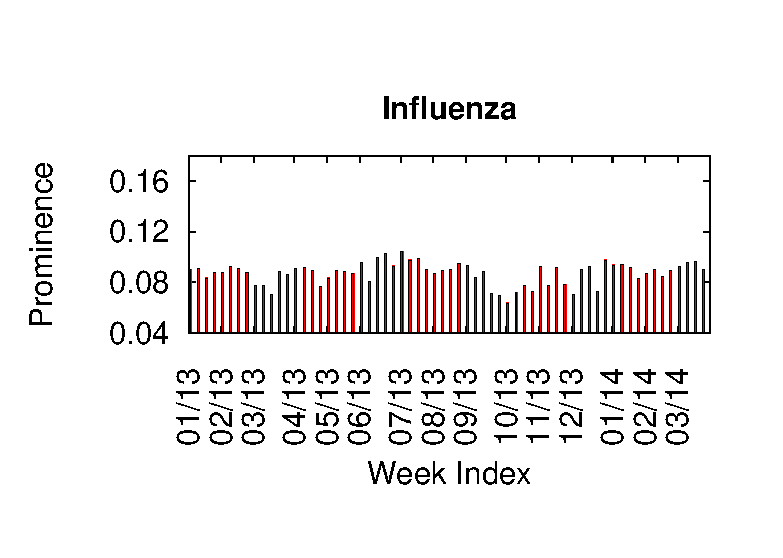
\includegraphics[clip,scale=0.45]{fig/topic_influenza_timeline.eps}} & \multicolumn{2}{|c|}{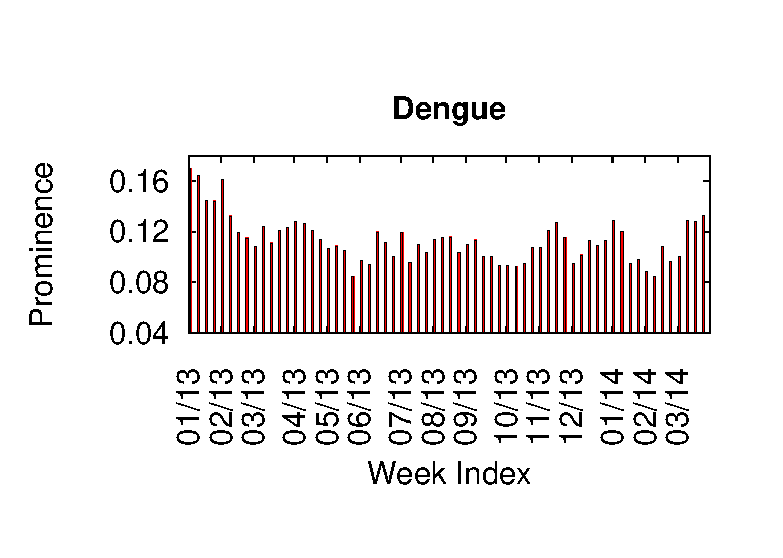
\includegraphics[clip,scale=0.45]{fig/topic_dengue_timeline.eps}}& 
\multicolumn{2}{|c|}{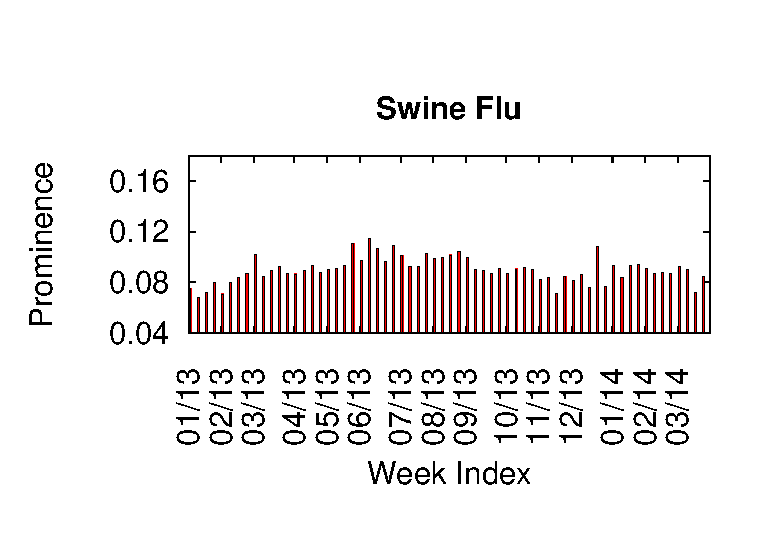
\includegraphics[clip,scale=0.45]{fig/topic_swine_timeline.eps}} \\ \hline
influenza & 0.0567 & dengue & 0.2095 & gripe & 0.0522 \\
mosquito & 0.0495 & aegypti & 0.0166 & h1n1 & 0.0351 \\
pacientes & 0.0258 & agua & 0.0137  & infectadas &0.0043 \\
aviar & 0.0144 & mosquitos & 0.0058  & flu & 0.0024\\
larvas & 0.0096 & agricultura & 0.0019 & bacteria & 0.0021 \\
fiebre & 0.0088 & respiratoria & 0.0018 & enfermo & 0.0008 \\
surto & 0.0061 & rurales & 0.0006 & vacinas & 0.0008 \\
zancudos & 0.0008 & agropecuario	 & 0.0006 & nasal & 0.0008 \\
avian & 0.0006 & hemorragias & 0.0005 & paracetamol & 0.0007 \\
h5n1 & 0.0003 & suero & 0.0004 & swine & 0.0005 \\
\hline
\end{tabular}\label{tab:common_topics}
\end{center}
\end{table*}

We evaluate the performance of the proposed topic model at discovering common disease topics and their temporal patterns. \Cref{tab:common_topics} shows three topics related to avian flu, dengue and swine flu. Again, we present their most likely words and their prominence histograms over time. For all three topics we see that the corresponding disease keywords, i.e., ``influenza",  ``dengue" and ``gripe" (flu) are ranked first. For the avian influenza topic, the proposed topic model is able to discover the correlation among words referring to both the {\em causes}, i.e., ``mosquito", ``larvas", ``zancudos" (mosquitos), and the {\em symptoms}, i.e., ``fiebre" (fever), of the disease. Regarding the dengue topic, our approach is able to identify the main transmission root of dengue which is via the aides aegypti mosquito, as well as, the fact that dengue is more prominent in rural and agricultural areas. Finally, a similar performance is observed for the swine flu topic. Our approach can identify the correlation between the word ``bacteria" and swine flu - bacteria co-infections play a key role in swine flu deaths - and the correlation between ``paracetamol" and swine flu, one of indicated medication substances for the disease.

\section{How effective is the proposed topic model in identifying spatial patterns?} 
\label{sec:spatial}
We examine the correlations between the discovered topics and the countries in Latin America under consideration. \Cref{fig:country_topic} shows the prominence of each topic for Brazil, Chile, Uruguay and Argentina. As expected, we observe that in Chile, HPS and HFRS are more prominent compared to other countries.

\begin{figure}[h]
\begin{center}
	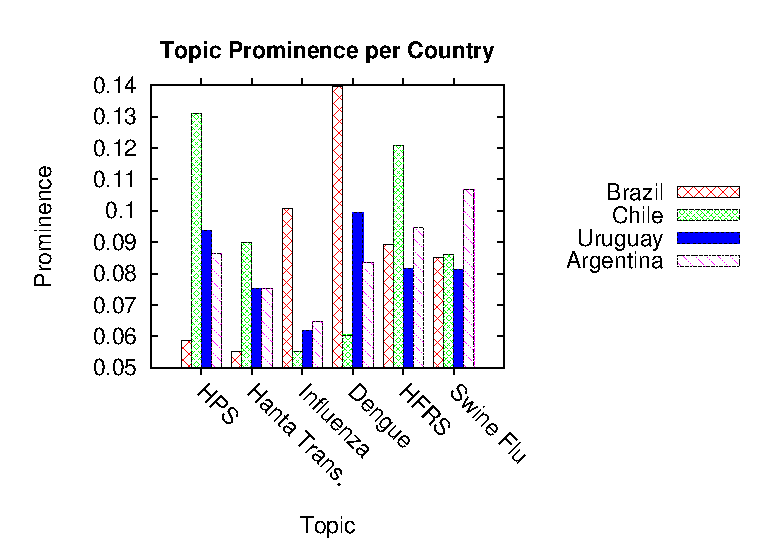
\includegraphics[trim=5 0 10 10, clip,scale=0.6]{fig/country_topic.eps}
\end{center}
 \vspace{-10pt}
\caption{The country specific topic prominence for different diseases. The numbers reported are averaged over all states corresponding to each country.}
 \label{fig:country_topic}
 \vspace{-10pt}
\end{figure}


\section{ Evaluation of Different Prediction Approaches}
\label{sec:full_eval}
In this section, we present the detailed evaluation results for the performance of BSR, \keymodel, \locationmodel, and \fullmodel on predicting Hantavirus incidences from January 2013 to March 2014. \Cref{tab:results} shows the precision, recall and F1 score  of the four approaches aggregated over Chile, Argentina, Brazil and Uruguay. For \locationmodel and \fullmodel we report the results for the configuration $k$ that obtained the best performance. 

\begin{table*}[ht]
\scriptsize \centering
  \caption{BSR, \keymodel, \locationmodel and \fullmodel on predicting hantavirus outbreaks. Notation $(k\% )$ denotes the best performing configuration for \locationmodel and \fullmodel. }
  \begin{tabular}{|c|c|c|c|c|c|c|c|c|c|c|c|c|}
    \hline
    & \multicolumn{3}{c|}{{\bf BSR}} &
    \multicolumn{3}{c|}{{\bf \keymodel}} &
    \multicolumn{3}{c|}{{\bf \locationmodel(5\%)}} &
    \multicolumn{3}{c|}{{\bf \fullmodel(5\%)}} \\
    \cline{2-10} {\em Month}   & {\em Prec.} & {\em Rec.} & {\em F1} & {\em Prec.} & {\em Rec.} & {\em F1} & {\em Prec.} & {\em Rec.} & {\em F1} & {\em Prec.} & {\em Rec.} & {\em F1} \\
    \hline 
    01/13 & 0.5 & 0.17 & 0.25 & {\bf 0.67}& 0.33& 0.44& 0.13 & {\bf 0.67} & 0.22 & 0.44 & {\bf 0.67} & {\bf 0.53}\\ 
    \hline
     02/13 & 0.52 & 0.78 & 0.62 & {\bf 0.67} & {\bf 1.0}& {\bf 0.80} & 0.12 & {\bf 1.0} & 0.21 & 0.5 & {\bf 1.0} & 0.67\\ 
    \hline
    03/13 & {\bf 0.7} & 0.35 & 0.46 & 0.6 & {\bf 0.75} & {\bf 0.67} & 0.29 & 0.5 & 0.37 & 0.5 & 0.5 & 0.5\\ 
    \hline
    04/13 & {\bf 0.78} & 0.59 & 0.67 & 0.33  & 0.25  & 0.28 & 0.6 & 0.75 & 0.67 & 0.57 & {\bf 1.0} & {\bf 0.73}\\ 
    \hline
    05/13 & {\bf 0.51} & 0.48 & {\bf 0.54} & 0.29 & 0.4 & 0.34& 0.14 & 0.2 & 0.16 & 0.38 & {\bf 0.6} & 0.47\\ 
    \hline
    06/13 & {\bf 0.22} & 0.68 & {\bf 0.33} & 0& 0& 0& 0.14 & {\bf 1.0} & 0.25 & 0.14 & {\bf 1.0} & 0.25\\ 
    \hline
    07/13 & {\bf 0.22} & 0.68 & {\bf 0.33} & 0& 0& 0& 0.14 & {\bf 1.0} & 0.25 & 0.2 & {\bf 1.0} & {\bf 0.33}\\ 
    \hline
    08/13 & 0.4 & 0.6 & 0.47 & 0& 0& 0& 0.2 & {\bf 1.0} & 0.33 & {\bf 0.67} & {\bf 1.0} & {\bf 0.80}\\ 
    \hline
    09/13 & 0.5 & 0.33 & 0.39 & 0& 0& 0& 0.23 & {\bf 1.0} & 0.37 & {\bf 0.67} & {\bf 0.67} & {\bf 0.67}\\ 
    \hline
    10/13 & {\bf 0.62} & 0.24 & 0.35 & 0.5& 0.4& 0.44& 0.31 & {\bf 0.8} & 0.45 & 0.38 & 0.6 & {\bf 0.47}\\ 
    \hline
    11/13 & {\bf 0.89} & 0.44 & 0.59 & 0.75& 0.5& {\bf 0.6}& 0.21 & {\bf 0.83} & 0.34 & 0.45 & {\bf 0.83} & 0.58\\ 
    \hline
    12/13 & 0.9 & 0.32 & 0.47 & {\bf 0.75}& 0.27& 0.40& {\bf 0.75} & {\bf 0.55} & {\bf 0.63} & 0.67 & {\bf 0.55} & 0.60\\ 
    \hline
    01/14 & 0.65 & 0.49 & 0.56 & 0.43& 0.38& 0.40& 0.19 & 0.5 & 0.28 &  {\bf 0.71}& {\bf 0.63} & {\bf 0.67}\\ 
    \hline
    02/14 & 0.56 & {\bf 0.74} & 0.64 & 0.43 & 0.5 & 0.46 & 0.27 &  0.67 & 0.38 & {\bf 0.67} & 0.67 & {\bf 0.67}\\ 
    \hline
    03/14 & 0.55 & {\bf 0.88} & {\bf 0.68} & {\bf 0.57} & 0.8& 0.66& 0.29 & 0.8 & 0.42 & 0.5 & 0.8 & 0.62 \\ 
    \hline
  \end{tabular}
  \vspace{-10pt}
  \label{tab:results}
\end{table*}

As shown, \fullmodel  obtains the best F1-score and recall for most of the months. We observe that the recall obtained by \locationmodel is comparable to that of \fullmodel, while the recall of BSR is significantly lower compared to that of both \locationmodel and \fullmodel. The latter is expected as BSR can only predict outbreaks for states where a sufficient number of outbreaks has occurred in the past. In fact, due to its design BSR fails completely to forecast outbreaks for states or countries where no outbreaks have been observed in the past (e.g., the outbreak in Brazil for October 2013 and the outbreak in Uruguay for March 2013).  However this mechanism limits the number of false positives significantly, and thus, for many months we observe slightly higher or comparable precision scores for BSR with those of \fullmodel. On the other hand the precision scores of \locationmodel are significantly lower compared to \fullmodel. The reason for this behavior is the increased number of false positives returned by \locationmodel even after the thresholding mechanism was employed. Regarding \keymodel, we observe that the model performs reasonably well when there is an increase in the number of outbreaks in previous weeks leading to increased keyword counts. However, the model performs poorly for cases when a small number of events was observed in the previous weeks. For example \keymodel failed to forecast Hantavirus outbreaks in August  and September 2013 because there was only one incidence in July. 



\end{document}
